
\documentclass[12pt]{article}

\usepackage{my-template}

% Disable indentation on new paragraphs
\setlength{\parindent}{0pt}

% Line spacing 1.5
% \renewcommand{\baselinestretch}{1.5}

% Optional: graphic path
% \graphicspath{PATH_TO_GRAPHIC_FOLDER}

% To use Times font family, uncomment this row
% \usepackage{mathptmx}

% To use roman section / subsection, uncomment these rows
% \renewcommand{\thesection}{\Roman{section}}
% \renewcommand{\thesubsection}{\thesection.\Roman{subsection}}

% Define course name, report name and report title.
\newcommand{\coursename}{Xử Lý Số Liệu Thống Kê}
\newcommand{\reportname}{ĐỒ ÁN CUỐI KÌ}
\newcommand{\reporttitle}{Phân tích và dự đoán xác suất kết thúc session từ dữ liệu clickstream}

% TODO: điền mã số học viên và họ tên đầy đủ của Nghi vào dòng thứ ba.
\newcommand{\studentname}
{
25C23002 & Nguyễn Nhật Quang\\
25C23014 & Lê Hoàng Như\\
25C230XX & Nghi\\

}

\newcommand{\teachername}{TS. Tô Đức Khánh}

% Header
% \lhead{\reporttitle}
% \rhead{
%   Trường Đại học Khoa học Tự nhiên - ĐHQG HCM\\
%   \coursename
% }

\usepackage{tikz}

% Bảng T5 của gói vietnam có thể thiếu dấu ogonek (ą) trong tên tác giả Ba Lan.
% Nếu \k chưa được định nghĩa, in ra nguyên chữ cái thay vì báo lỗi biên dịch.
\providecommand{\k}[1]{#1}

% Bảng dài có thể ngắt trang và bảng rộng xoay ngang.
\usepackage{longtable}
\usepackage{multirow}
\usepackage{pdflscape}
\usepackage{caption}
\captionsetup[table]{skip=4pt}
\captionsetup[figure]{skip=4pt}

% Footer
% \newcommand{\leftfooter}{\LaTeX\ by \href{https://github.com/trhgquan}{Quan, Tran Hoang}}
% \lfoot{\leftfooter}
% ============ DOCUMENT ============
\begin{document}
\pagenumbering{roman}
\input{content/title.tex}

\tableofcontents
\thispagestyle{empty}
\pagebreak

\listoftables
\thispagestyle{empty}
\pagebreak

\listoffigures
\thispagestyle{empty}
\pagebreak

\pagenumbering{arabic}
\setcounter{page}{1}

% Nội dung phần 1: Giới thiệu chung và bản đề xuất phân tích.

\section{Giới thiệu chung và bản đề xuất phân tích}

\subsection{Giới thiệu bộ dữ liệu}

Bộ dữ liệu \textbf{e-shop clothing 2008} ghi nhận toàn bộ hành vi click trên một
cửa hàng quần áo trực tuyến của Ba Lan trong năm 2008. Mỗi dòng dữ liệu là một
lượt click; các click có cùng \texttt{session\_id} tạo thành một phiên duyệt web
và biến \texttt{order} cho biết vị trí của click trong phiên đó. Dữ liệu được
công bố kèm nghiên cứu của {\L}apczy\'nski và Bia{\l}ow{\k a}s
(2013)~\cite{lapczynski2013} về hành vi người dùng trong cửa hàng trực tuyến, và
hiện được lưu trữ tại UCI Machine Learning Repository~\cite{uci_clickstream}.

Nhóm chọn bộ dữ liệu này vì ba lý do. Thứ nhất, quy mô đủ lớn (165.474 click của
24.026 session) để tách tập huấn luyện và tập kiểm tra theo thời gian mà vẫn còn
đủ quan sát. Thứ hai, dữ liệu có cấu trúc tuần tự theo session, cho phép đặt một
câu hỏi thống kê phi tầm thường thay vì chỉ mô tả. Thứ ba, dữ liệu kết hợp cả
biến liên tục (giá) lẫn nhiều biến phân loại (danh mục, màu sắc, vị trí ảnh,
trang hiển thị), phù hợp để so sánh hồi quy tuyến tính, GLM và GAM trên cùng một
bài toán.

\begin{table}[H]
\centering
\caption{Tổng quan bộ dữ liệu}
\label{tab:overview}
\begin{tabular}{ll}
\toprule
\textbf{Chỉ tiêu} & \textbf{Giá trị} \\
\midrule
Số click              & 165.474 \\
Số session            & 24.026 \\
Số quốc gia / mã miền & 47 \\
Số sản phẩm           & 217 \\
Số danh mục           & 4 \\
Khoảng thời gian      & 01/04/2008 -- 13/08/2008 \\
Tỷ lệ Continue        & 85,48\% \\
Tỷ lệ Exit            & 14,52\% \\
\bottomrule
\end{tabular}
\end{table}

Bên cạnh các ưu điểm trên, dữ liệu cũng có giới hạn cần nêu ngay từ đầu vì nó
quyết định phạm vi kết luận: không có thông tin giao dịch, giỏ hàng hay thanh
toán; không có giờ click và thời lượng giữa hai click; và tháng 8 chỉ được thu
thập đến ngày 13, trong đó riêng ngày 13/08 chỉ có 200 click. Vì vậy không thể so
sánh tổng lưu lượng tháng 8 trực tiếp với các tháng đầy đủ.

\subsection{Ý nghĩa các biến và biến mục tiêu}

Bảng~\ref{tab:vardict} tóm tắt ý nghĩa và vai trò của từng biến trong phân tích.
Có ba điểm dễ hiểu sai cần lưu ý: \texttt{location} là vị trí của \emph{bức ảnh}
trong sáu vùng của trang web chứ không phải vị trí địa lý của khách hàng;
\texttt{category} tương ứng cột \texttt{PAGE 1} (danh mục chính) còn
\texttt{page} tương ứng cột \texttt{PAGE} (số trang hiển thị 1--5); biến
\texttt{year} bị loại vì chỉ nhận một giá trị duy nhất nên không có biến thiên.

\begin{table}[H]
\centering
\caption{Từ điển biến và vai trò trong phân tích}
\label{tab:vardict}
\footnotesize
\begin{tabular}{>{\raggedright\arraybackslash}p{0.15\textwidth}
                >{\raggedright\arraybackslash}p{0.35\textwidth}
                >{\raggedright\arraybackslash}p{0.40\textwidth}}
\toprule
\textbf{Biến} & \textbf{Ý nghĩa} & \textbf{Vai trò} \\
\midrule
year, month, day & Ngày lịch; không có giờ hoặc thời lượng & Tạo \texttt{time\_30}; \texttt{year} bị loại vì không biến thiên \\[2pt]
order & Thứ tự click trong session & Predictor, dùng $\log_2(\text{order})$ hoặc hàm trơn \\[2pt]
country & Quốc gia hoặc loại tên miền của IP & Predictor factor; mức hiếm được gộp trên train \\[2pt]
session\_id & Mã session & Nhóm dữ liệu và tính robust SE; không làm predictor \\[2pt]
category & PAGE 1: trousers, skirts, blouses hoặc sale & Predictor factor \\[2pt]
product\_model & PAGE 2: mã của 217 sản phẩm & Không đưa vào mô hình chính do có 217 mức \\[2pt]
colour & Màu sản phẩm & Predictor factor \\[2pt]
location & Vị trí ảnh trong sáu vùng của trang; không phải địa lý & Predictor factor \\[2pt]
photography & Kiểu ảnh en face hoặc profile & Predictor factor \\[2pt]
price & Giá sản phẩm, USD & Predictor liên tục \\[2pt]
price\_above\_avg & 1 = cao hơn trung bình danh mục; 2 = không & Tạo hai nhóm cho kiểm định; không dùng cùng \texttt{price} trong mô hình A/B \\[2pt]
page & Trang hiển thị trong website, từ 1 đến 5 & Predictor factor \\
\bottomrule
\end{tabular}
\end{table}

Bộ dữ liệu gốc không có sẵn biến mục tiêu. Nhóm định nghĩa target thống nhất cho
mọi mô hình xác suất trong báo cáo là biến nhị phân \texttt{Exit}:

\[
Exit_{it} =
\begin{cases}
1, & \text{click hiện tại là click cuối của session;}\\
0, & \text{session còn click tiếp theo.}
\end{cases}
\]

Biến \texttt{session\_length} chỉ được dùng để \emph{tạo} target và tuyệt đối
không được đưa vào tập predictor, vì tại thời điểm click thứ $t$ độ dài cuối cùng
của session là thông tin tương lai. Đại lượng được nghiên cứu vì vậy là một xác
suất nguy cơ rời rạc (discrete-time hazard):

\[
P\{Exit_{it}=1\mid \text{session đã tiếp tục đến click }t\}.
\]

Tại \texttt{order} $=t$, mẫu số chỉ gồm các session còn tồn tại đến click $t$.
Do đó mọi kết quả theo \texttt{order} là quan hệ \emph{có điều kiện} trên nhóm
session còn sống sót, không phải bằng chứng rằng việc tăng số click gây ra thay
đổi nguy cơ kết thúc.

\subsection{Các mục tiêu phân tích}

\begin{enumerate}
  \item \textbf{So sánh hai nhóm dạng A/B.} Kiểm định xem xác suất \texttt{Exit}
  có khác nhau giữa click vào sản phẩm có giá cao hơn trung bình danh mục
  (nhóm B) và click vào sản phẩm không cao hơn trung bình (nhóm A) hay không.

  \item \textbf{Phân tích các yếu tố liên quan đến \texttt{Exit}.} Mô tả quan hệ
  giữa xác suất kết thúc và tiến trình session; đánh giá xem đặc điểm của click
  hiện tại và lịch sử duyệt đã quan sát có bổ sung thông tin dự báo hay không.

  \item \textbf{Xây dựng và so sánh mô hình.} So sánh Linear Probability Model
  (LPM), Logistic GLM và Binomial GAM về khả năng phân biệt, chất lượng xác suất
  dự đoán, calibration và khả năng diễn giải.
\end{enumerate}

Cần nhấn mạnh một điểm về thiết kế: nhóm giá \emph{không} được gán ngẫu nhiên cho
người dùng mà là một thuộc tính sẵn có của sản phẩm. Vì vậy Mục tiêu 1 là một so
sánh hai nhóm \textbf{dạng A/B trên dữ liệu quan sát}, không phải một thí nghiệm
A/B có treatment và control. Mọi kết luận rút ra chỉ phản ánh mối liên hệ, không
phải quan hệ nhân quả.

\subsection{Phương pháp và chiến lược phân tích}

\subsubsection{Chiến lược cho Mục tiêu 1}

Giả thuyết được phát biểu hai phía tại mức ý nghĩa $\alpha = 0{,}05$:
\[
H_0: P(Exit=1\mid A)=P(Exit=1\mid B),
\qquad
H_1: P(Exit=1\mid A)\ne P(Exit=1\mid B).
\]
Các bước thực hiện gồm: (i) tính tỷ lệ \texttt{Exit} thô và khoảng tin cậy
Wilson~\cite{wilson1927} cho từng nhóm; (ii) ước lượng risk difference thô kèm
khoảng tin cậy cluster-bootstrap theo session; (iii) ước lượng adjusted odds
ratio và adjusted risk difference từ mô hình logistic có kiểm soát tiến trình
session, thời gian, country và đặc điểm sản phẩm, với sai số chuẩn
cluster-robust theo \texttt{session\_id}~\cite{zeileis2004, cameron2015};
(iv) kiểm tra balance giữa hai nhóm bằng standardized mean difference;
(v) kiểm tra dị biệt hiệu ứng theo \texttt{category} với hiệu chỉnh đa kiểm định
Holm~\cite{holm1979}; (vi) lặp lại phân tích trên ba giai đoạn thời gian để đánh
giá độ ổn định.

\subsubsection{Chiến lược cho Mục tiêu 2 và Mục tiêu 3}

Ba tầng predictor được so sánh trên cùng một pipeline:

\begin{itemize}
  \item \textbf{Baseline:} $\log_2(\texttt{order}) + \texttt{time\_30} + \texttt{country}$.
  \item \textbf{Current-click:} thêm \texttt{price}, \texttt{category},
  \texttt{colour}, \texttt{location}, \texttt{photography} và \texttt{page}.
  \item \textbf{History-enhanced:} thêm số sản phẩm và số danh mục duy nhất đã
  xem, cờ quay lại sản phẩm cũ, cờ chuyển danh mục và chuyển trang, chênh lệch
  giá so với click trước và so với trung bình lịch sử, tỷ lệ quay lại sản phẩm và
  tỷ lệ chuyển danh mục.
\end{itemize}

Mọi đặc trưng lịch sử tại click $t$ chỉ sử dụng dữ liệu từ click 1 đến $t$, nên
không rò rỉ thông tin tương lai. Biến \texttt{order} được đưa vào dưới dạng
$\log_2$ trong LPM và Logistic GLM, và dưới dạng hàm trơn $s(\cdot)$ trong
GAM~\cite{wood2017}, thay vì loại bỏ các session dài nằm ngoài râu boxplot. LPM
và Logistic GLM dùng cluster-robust covariance theo \texttt{session\_id}; GAM
dùng link logit với ước lượng fREML.

Việc chia dữ liệu được thực hiện theo thời gian chứ không ngẫu nhiên, để mô phỏng
đúng tình huống dự báo trong thực tế (Bảng~\ref{tab:split}).

\begin{table}[H]
\centering
\caption{Chia dữ liệu theo thời gian}
\label{tab:split}
\begin{tabular}{llrr}
\toprule
\textbf{Tập} & \textbf{Thời gian} & \textbf{Số click} & \textbf{Số session} \\
\midrule
Train              & Tháng 4--6 & 116.095 & 17.031 \\
Validation         & Tháng 7    & 35.231  & 5.071 \\
Temporal test      & 01--12/08  & 13.948  & 1.903 \\
Loại khỏi đánh giá & 13/08      & 200     & 21 \\
\bottomrule
\end{tabular}
\end{table}

Ngày 13/08 bị loại khỏi mọi đánh giá vì chỉ có 200 click, nhiều khả năng là ngày
thu thập chưa hoàn tất. Toàn bộ quy tắc tiền xử lý được học trên tập train: các
country có dưới 100 click trong train được gộp thành mức \texttt{Other}, rồi áp
dụng nguyên quy tắc đó cho validation và temporal test. Không có session nào xuất
hiện đồng thời trong hai tập bất kỳ, nên không có rò rỉ dữ liệu theo cụm.

Về đánh giá, do lớp \texttt{Exit} chiếm thiểu số (14,52\%), Accuracy không được
dùng làm tiêu chí chọn mô hình. Thay vào đó nhóm dùng ROC--AUC, Average
Precision, log loss, Brier score, Brier Skill Score và hai chỉ số calibration
(intercept và slope)~\cite{steyerberg2010}. Threshold tối đa hóa $F_1$ được chọn
từ prediction out-of-fold của five-fold cross-validation \emph{theo session} trên
tập train, và bị khóa lại trước khi chạm vào validation hay temporal test.
Tháng 7 được dùng để so sánh đặc tả và chọn mô hình; các ngày 01--12/08 chỉ được
mở đúng một lần ở cuối để báo cáo khả năng khái quát hóa.

%\newpage
% Nội dung phần 2: Khám phá và tổng hợp dữ liệu (EDA).

\section{Khám phá và tổng hợp dữ liệu}

\subsection{Làm sạch dữ liệu}

Trước khi phân tích, nhóm chạy một bộ kiểm tra chất lượng trên toàn bộ 165.474
dòng. Kết quả được tổng hợp ở Bảng~\ref{tab:quality}: không có giá trị khuyết
thiếu, không có dòng trùng lặp hoàn toàn, không có session nào bị đứt quãng thứ
tự \texttt{order}, mọi session đều có đúng một click mang nhãn \texttt{Exit}, và
không có session nào bị chia cắt giữa hai tập dữ liệu.

\begin{table}[H]
\centering
\caption{Kết quả kiểm tra chất lượng dữ liệu}
\label{tab:quality}
\begin{tabular}{lr}
\toprule
\textbf{Kiểm tra} & \textbf{Số trường hợp vi phạm} \\
\midrule
Giá trị khuyết thiếu                 & 0 \\
Dòng trùng hoàn toàn                 & 0 \\
Session có \texttt{order} không liên tục & 0 \\
Session không có đúng một \texttt{Exit}  & 0 \\
Session xuất hiện ở cả train và test     & 0 \\
\bottomrule
\end{tabular}
\end{table}

Về chuyển đổi kiểu dữ liệu, các cột mã số nguyên có bản chất phân loại được
chuyển thành factor kèm nhãn đọc được: \texttt{country} (47 mức),
\texttt{category} (4 mức), \texttt{colour} (14 mức), \texttt{location} (6 mức),
\texttt{photography} (2 mức) và \texttt{page} (5 mức). Ba cột
\texttt{year}, \texttt{month}, \texttt{day} được ghép thành một biến ngày, từ đó
tạo biến thời gian liên tục \texttt{time\_30} tính theo đơn vị 30 ngày kể từ ngày
đầu tiên của dữ liệu.

Về dữ liệu ngoại lai, nhóm \textbf{không} xóa và cũng không winsorize các session
dài, dù chúng nằm xa ngoài râu boxplot (\texttt{order} lớn nhất là 195). Lý do là
các session này có trình tự \texttt{order} hoàn toàn hợp lệ và phản ánh hành vi
duyệt dài có thật, không phải lỗi ghi nhận. Thay vì loại dữ liệu hợp lệ, nhóm xử
lý phần đuôi phải bằng phép biến đổi $\log_2(\texttt{order})$ trong LPM/Logistic
và bằng hàm trơn trong GAM.

\subsection{Thống kê mô tả}

Cần phân biệt hai đơn vị phân tích khác nhau. Phân phối \texttt{order} được tính
trên toàn bộ click, còn phân phối độ dài session được tính ở cấp session. Vì các
session dài đóng góp nhiều click hơn vào tổng thể, không được dùng trung vị
\texttt{order} trên click để kết luận về một session điển hình.

\begin{table}[H]
\centering
\caption{Thống kê mô tả các biến định lượng}
\label{tab:continuous}
\small
\begin{tabular}{llrrrrrrrr}
\toprule
\textbf{Biến} & \textbf{Đơn vị} & \textbf{N} & \textbf{Mean} & \textbf{Median}
& \textbf{Q1} & \textbf{Q3} & \textbf{Min} & \textbf{Max} & \textbf{SD} \\
\midrule
Price          & Click   & 165.474 & 43,80 & 43 & 33 & 52 & 18 & 82 & 12,55 \\
Order          & Click   & 165.474 & 9,82  & 6  & 2  & 12 & 1  & 195 & 13,48 \\
Session length & Session & 24.026  & 6,89  & 4  & 2  & 8  & 1  & 195 & 9,00 \\
\bottomrule
\end{tabular}
\end{table}

Giá sản phẩm chỉ nhận 20 mức rời rạc từ 18 đến 82 USD, nên phân phối có nhiều
đỉnh; việc trung bình (43,80) gần trung vị (43) \emph{không} đủ để kết luận biến
này tuân theo phân phối chuẩn. Ngược lại, độ dài session lệch phải rất mạnh:
trung vị chỉ 4 click trong khi trung bình là 6,89; có 2,48\% session dài hơn 30
click và 0,071\% session dài hơn 100 click.

\begin{table}[H]
\centering
\caption{Bảng tần số các biến phân loại chính}
\label{tab:categorical}
\small
\begin{tabular}{llrr}
\toprule
\textbf{Biến} & \textbf{Nhóm} & \textbf{Số click} & \textbf{Tỷ lệ} \\
\midrule
\multirow{4}{*}{Category}
 & Trousers & 49.742 & 30,06\% \\
 & Skirts   & 38.408 & 23,21\% \\
 & Blouses  & 38.577 & 23,31\% \\
 & Sale     & 38.747 & 23,42\% \\
\midrule
\multirow{6}{*}{Location}
 & Top left      & 34.532 & 20,87\% \\
 & Top middle    & 33.383 & 20,17\% \\
 & Top right     & 21.656 & 13,09\% \\
 & Bottom left   & 27.377 & 16,54\% \\
 & Bottom middle & 27.783 & 16,79\% \\
 & Bottom right  & 20.743 & 12,54\% \\
\midrule
\multirow{2}{*}{Photography}
 & En face & 122.439 & 73,99\% \\
 & Profile & 43.035  & 26,01\% \\
\midrule
\multirow{2}{*}{Price group}
 & A: Không cao hơn TB & 80.779 & 48,82\% \\
 & B: Cao hơn TB       & 84.695 & 51,18\% \\
\midrule
\multirow{5}{*}{Page}
 & Page 1 & 93.452 & 56,48\% \\
 & Page 2 & 41.037 & 24,80\% \\
 & Page 3 & 19.301 & 11,66\% \\
 & Page 4 & 8.861  & 5,35\% \\
 & Page 5 & 2.823  & 1,71\% \\
\bottomrule
\end{tabular}
\end{table}

Hai nhóm giá gần cân bằng về số lượng (48,82\% so với 51,18\%), thuận lợi cho
việc ước lượng chênh lệch với sai số chuẩn nhỏ. Tuy nhiên, cân bằng về \emph{cỡ
mẫu} không biến dữ liệu quan sát thành một thí nghiệm ngẫu nhiên -- điều này sẽ
được kiểm chứng bằng balance diagnostics ở Mục~\ref{subsec:ab}.

Phân phối \texttt{page} rất lệch: hơn một nửa số click nằm ở trang 1 và chỉ
1,71\% ở trang 5. Đây là lý do \texttt{page} được giữ ở dạng factor thay vì xem
như biến liên tục.

\subsection{Trực quan hóa dữ liệu}

\begin{figure}[H]
\centering
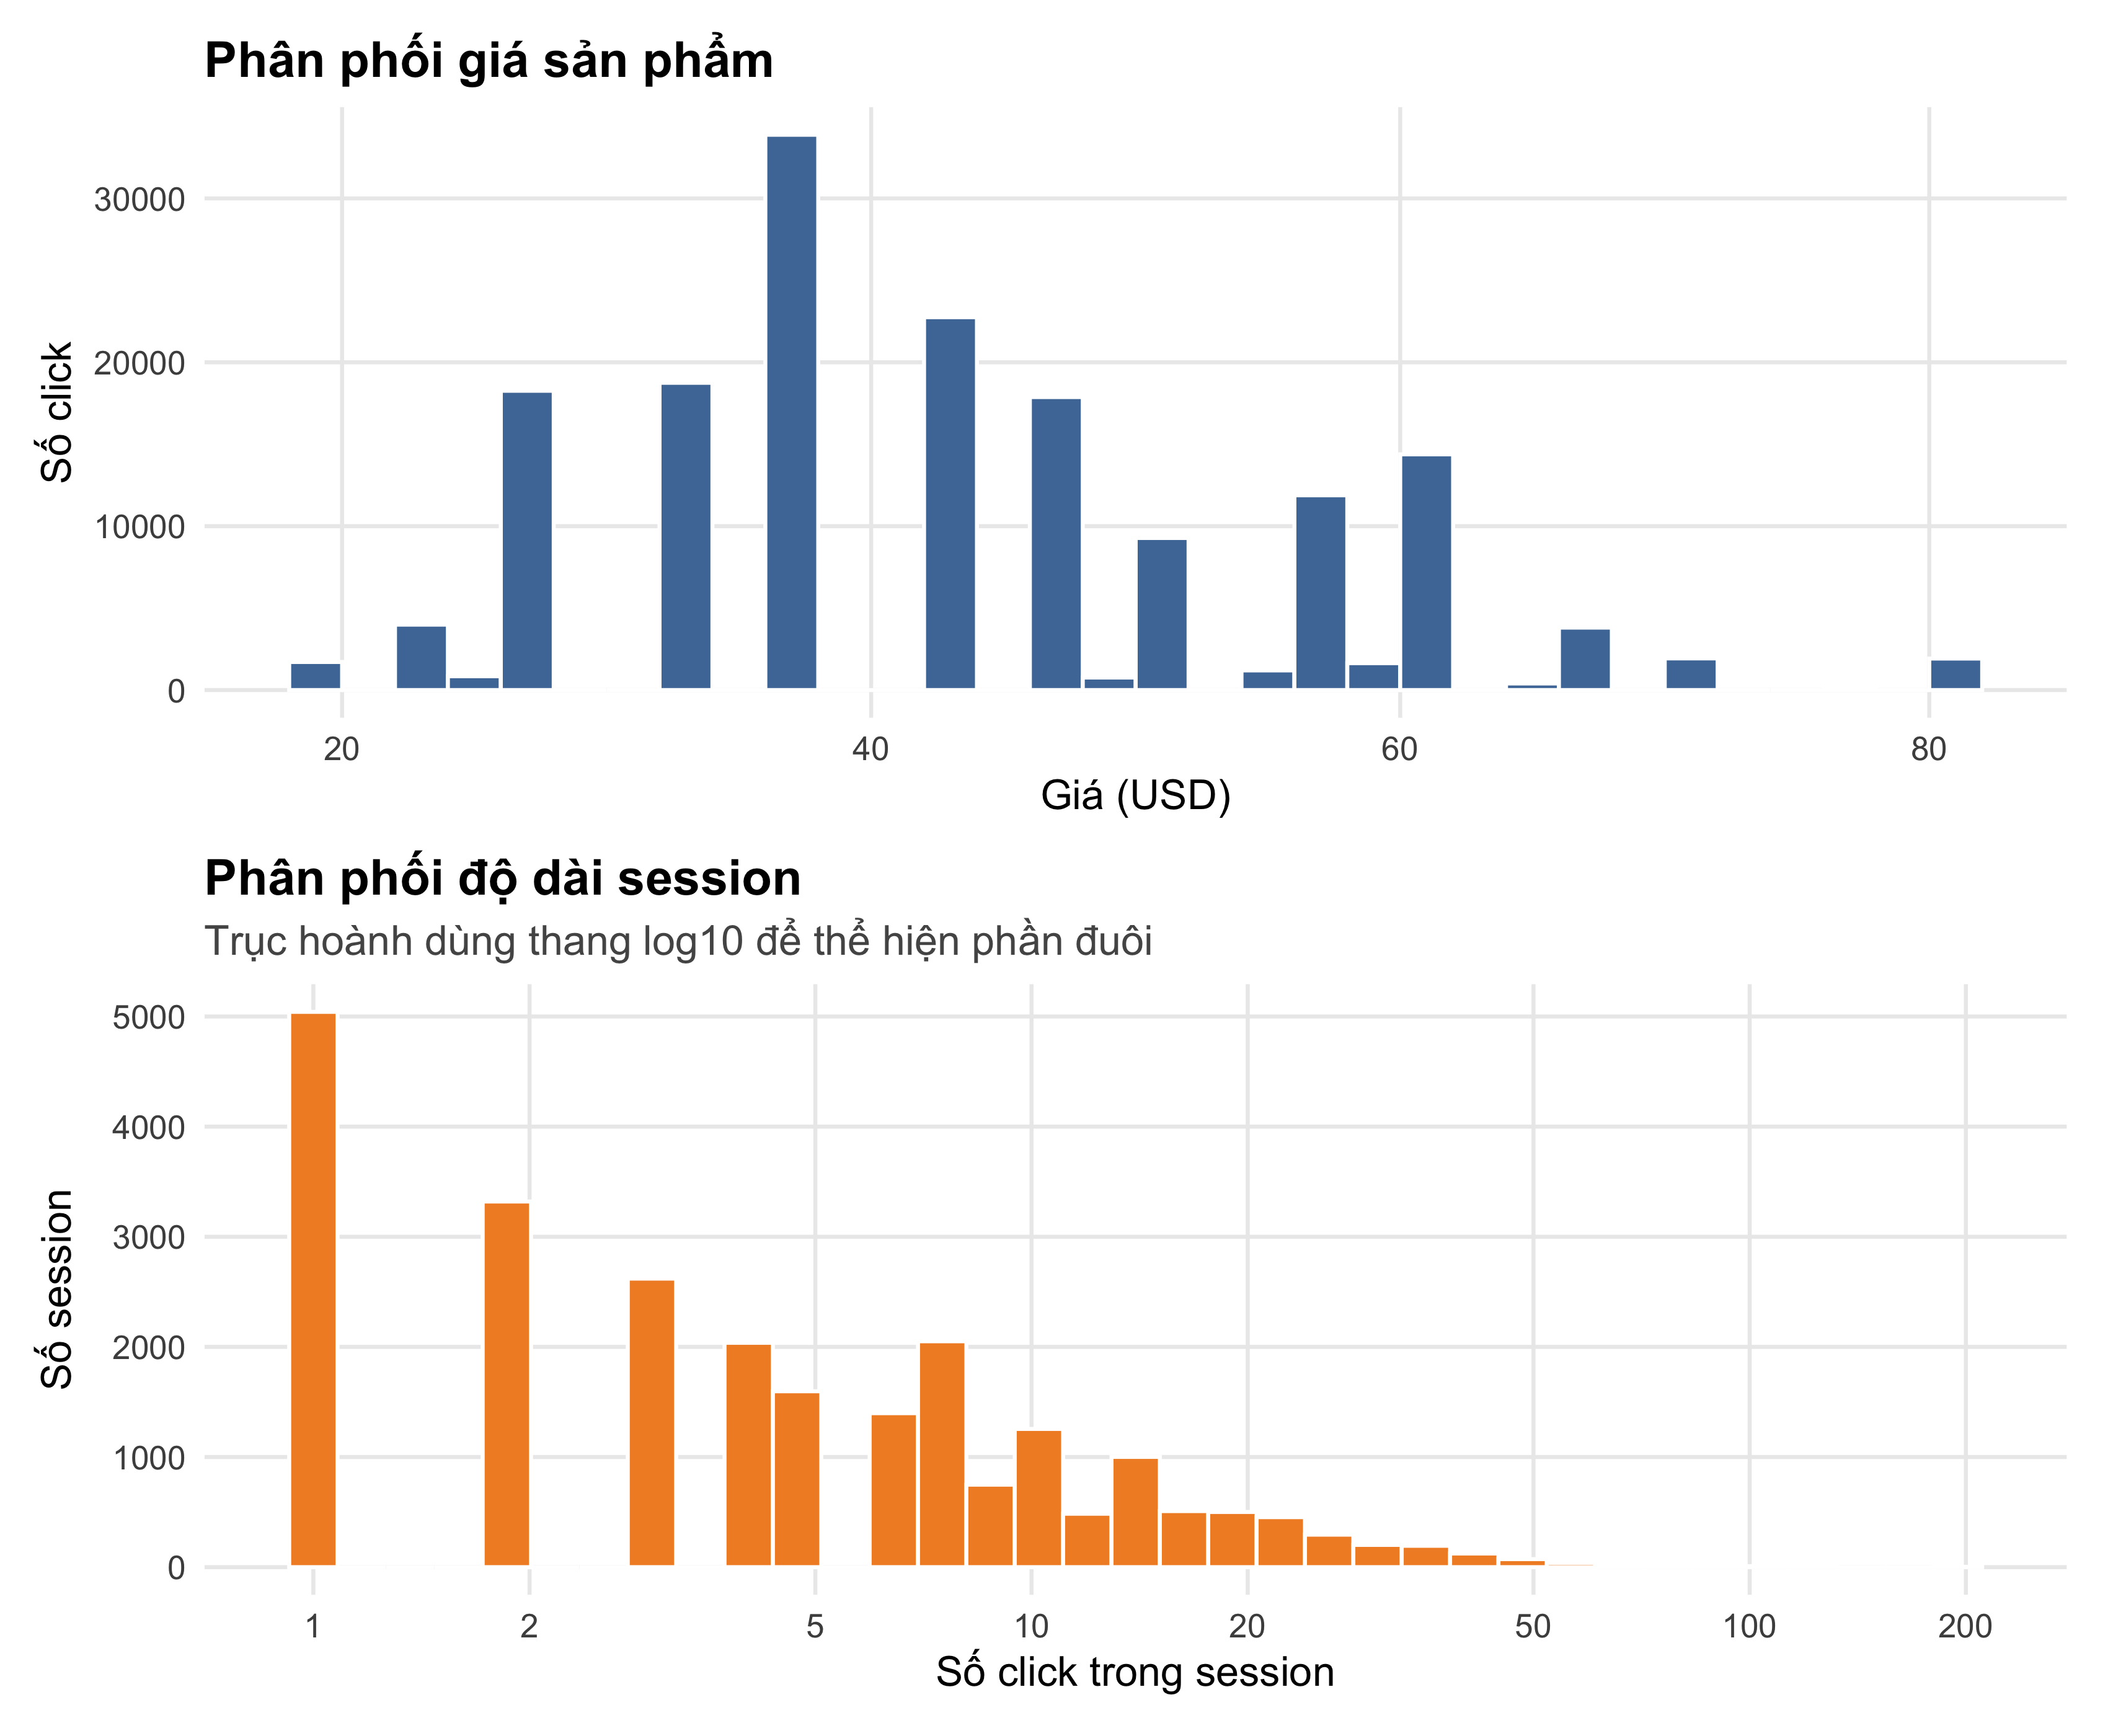
\includegraphics[width=\textwidth]{img/fig-eda-distributions.png}
\caption{Phân phối giá sản phẩm và phân phối độ dài session (trục hoành thang
log10)}
\label{fig:eda-distributions}
\end{figure}

Hình~\ref{fig:eda-distributions} cho thấy phân phối giá có dạng răng cưa, phản
ánh đúng bản chất rời rạc của các mức giá niêm yết. Phân phối độ dài session lệch
phải mạnh: phần lớn session rất ngắn, nhưng một tỷ lệ nhỏ kéo dài hàng chục đến
gần 200 click. Đây chính là căn cứ thực nghiệm cho quyết định dùng
$\log_2(\texttt{order})$ và hàm trơn thay vì cắt bỏ phần đuôi.

\begin{figure}[H]
\centering
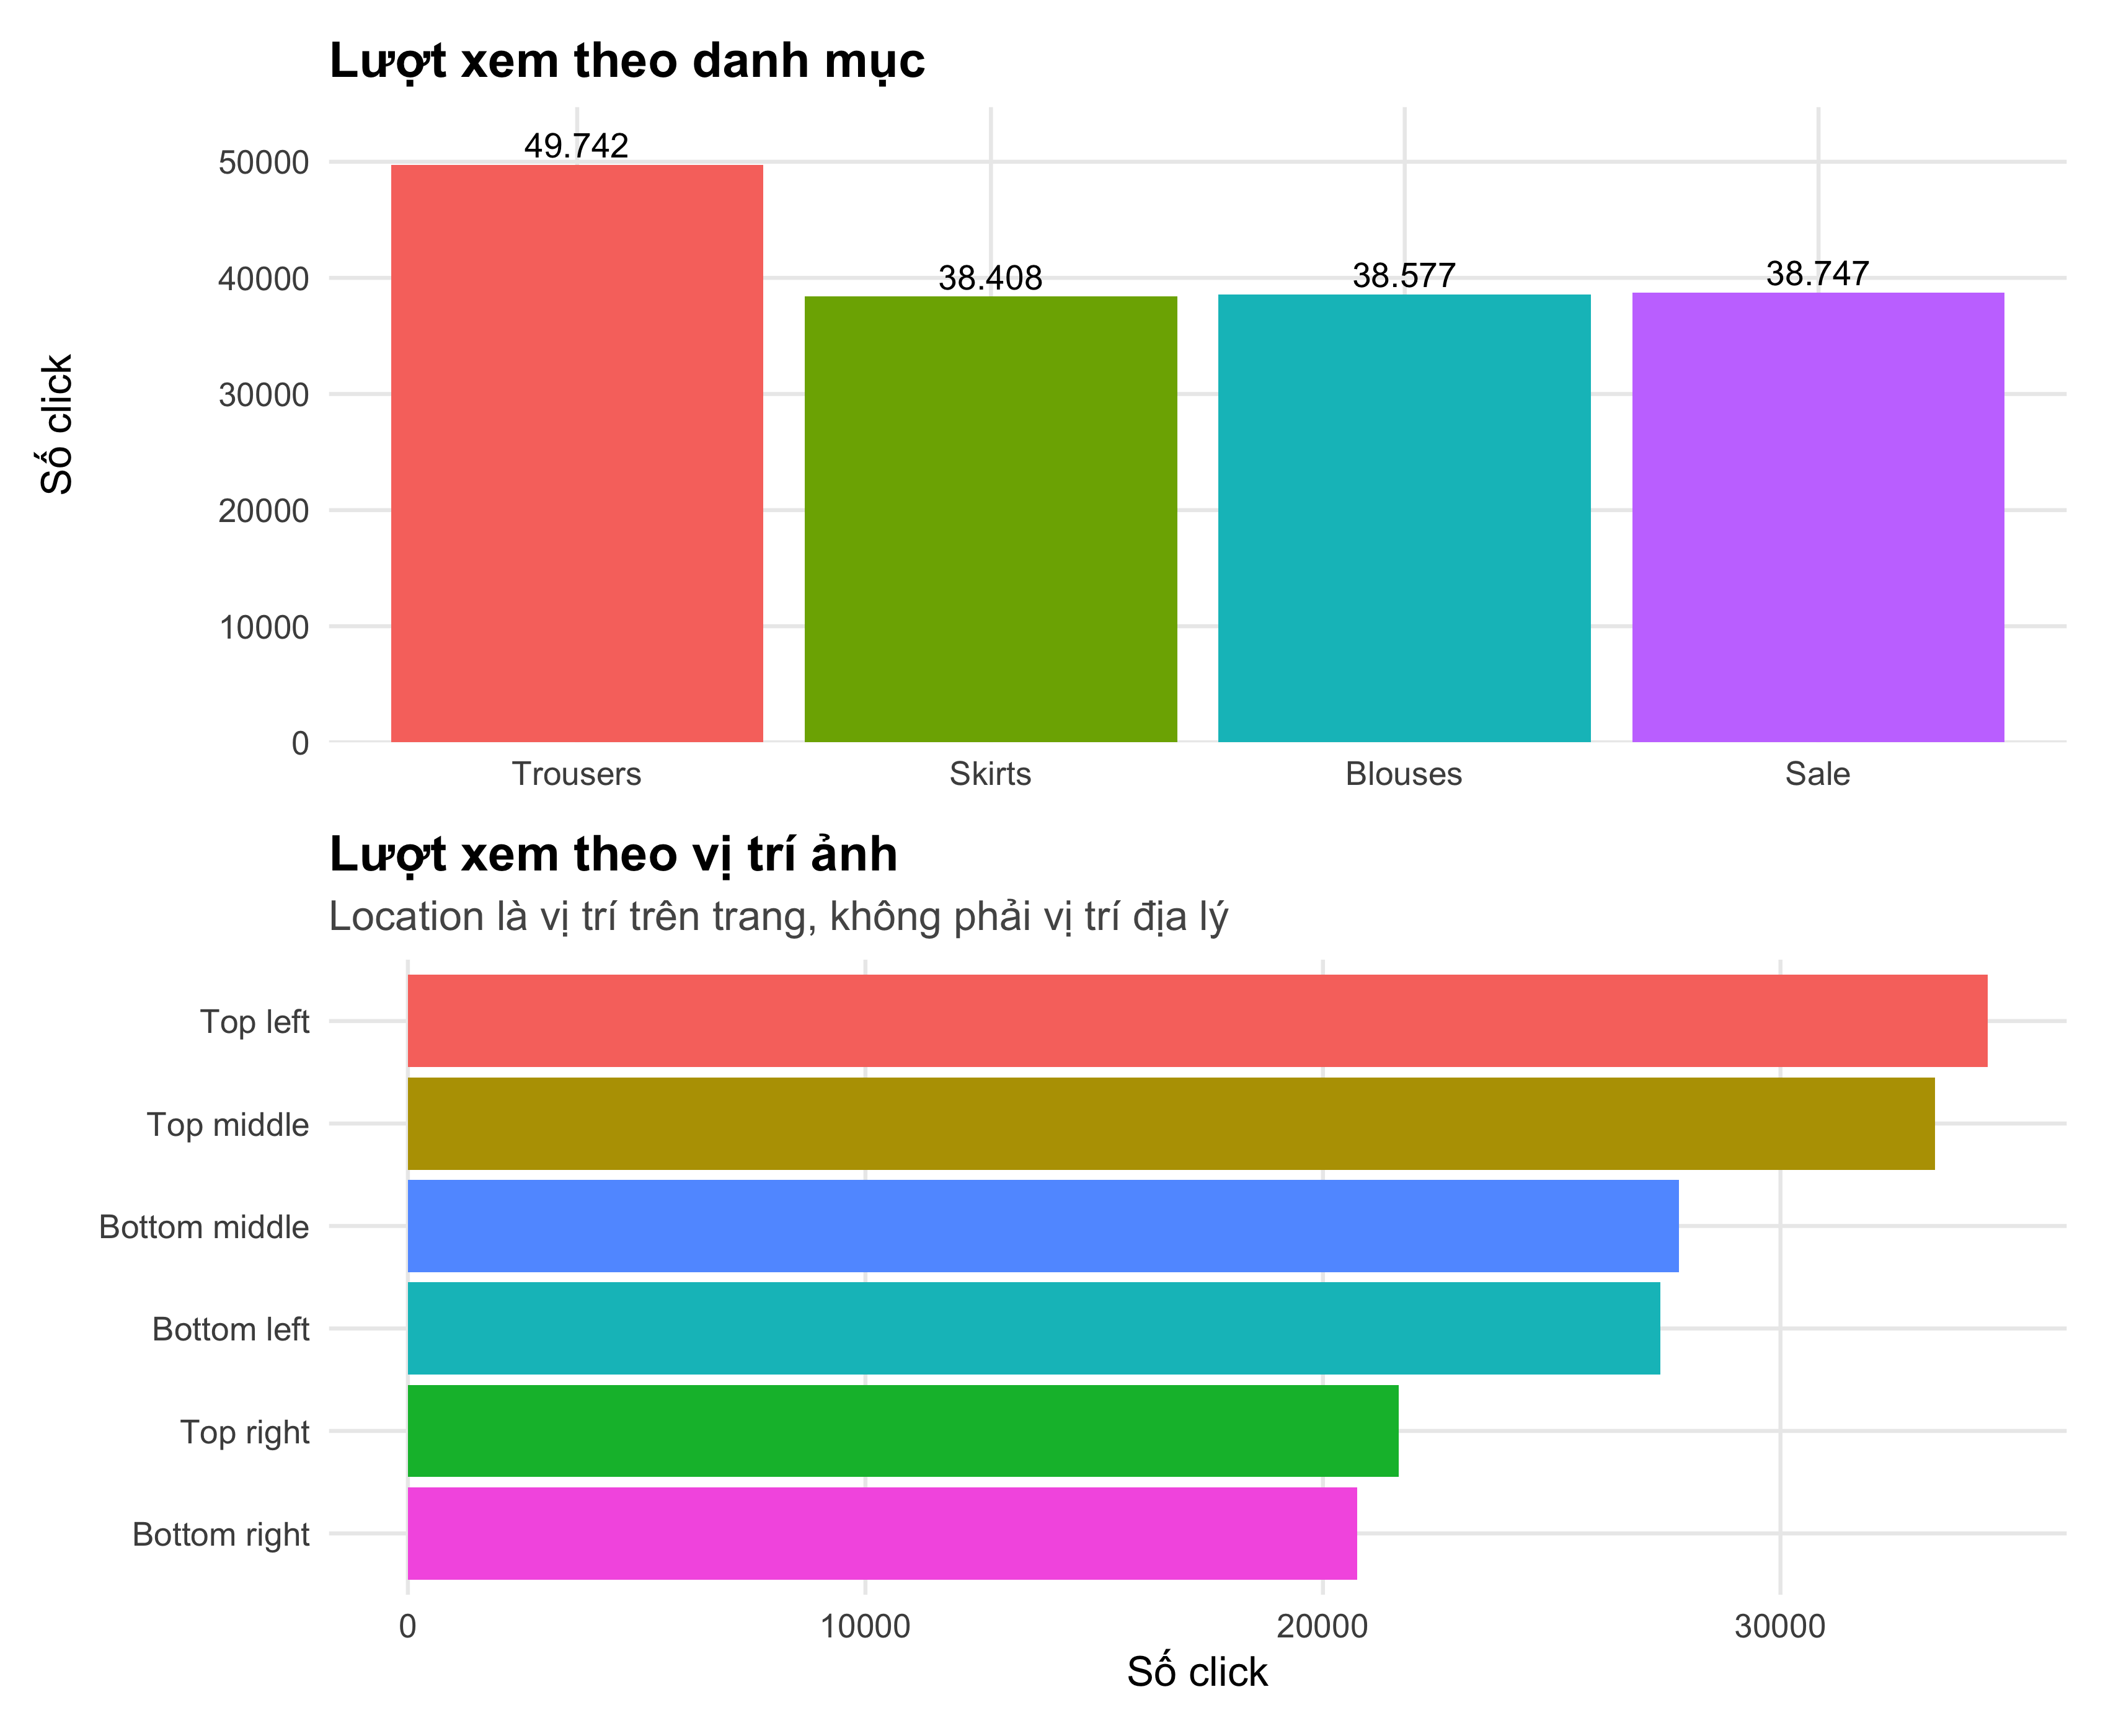
\includegraphics[width=\textwidth]{img/fig-eda-categories.png}
\caption{Số lượt click theo danh mục sản phẩm và theo vị trí ảnh trên trang}
\label{fig:eda-categories}
\end{figure}

Danh mục Trousers có số click cao hơn rõ rệt so với ba danh mục còn lại
(30,06\% so với khoảng 23\% mỗi nhóm). Đây chỉ là mô tả lưu lượng xem, chưa đủ để
kết luận danh mục này hấp dẫn hơn hay tạo chuyển đổi tốt hơn. Tương tự, các vị
trí ảnh có tần số khác nhau, nhưng vì mỗi mã sản phẩm chỉ xuất hiện tại một vị
trí cố định, khác biệt theo \texttt{location} có thể bị confounding hoàn toàn bởi
đặc điểm sản phẩm.

\begin{figure}[H]
\centering
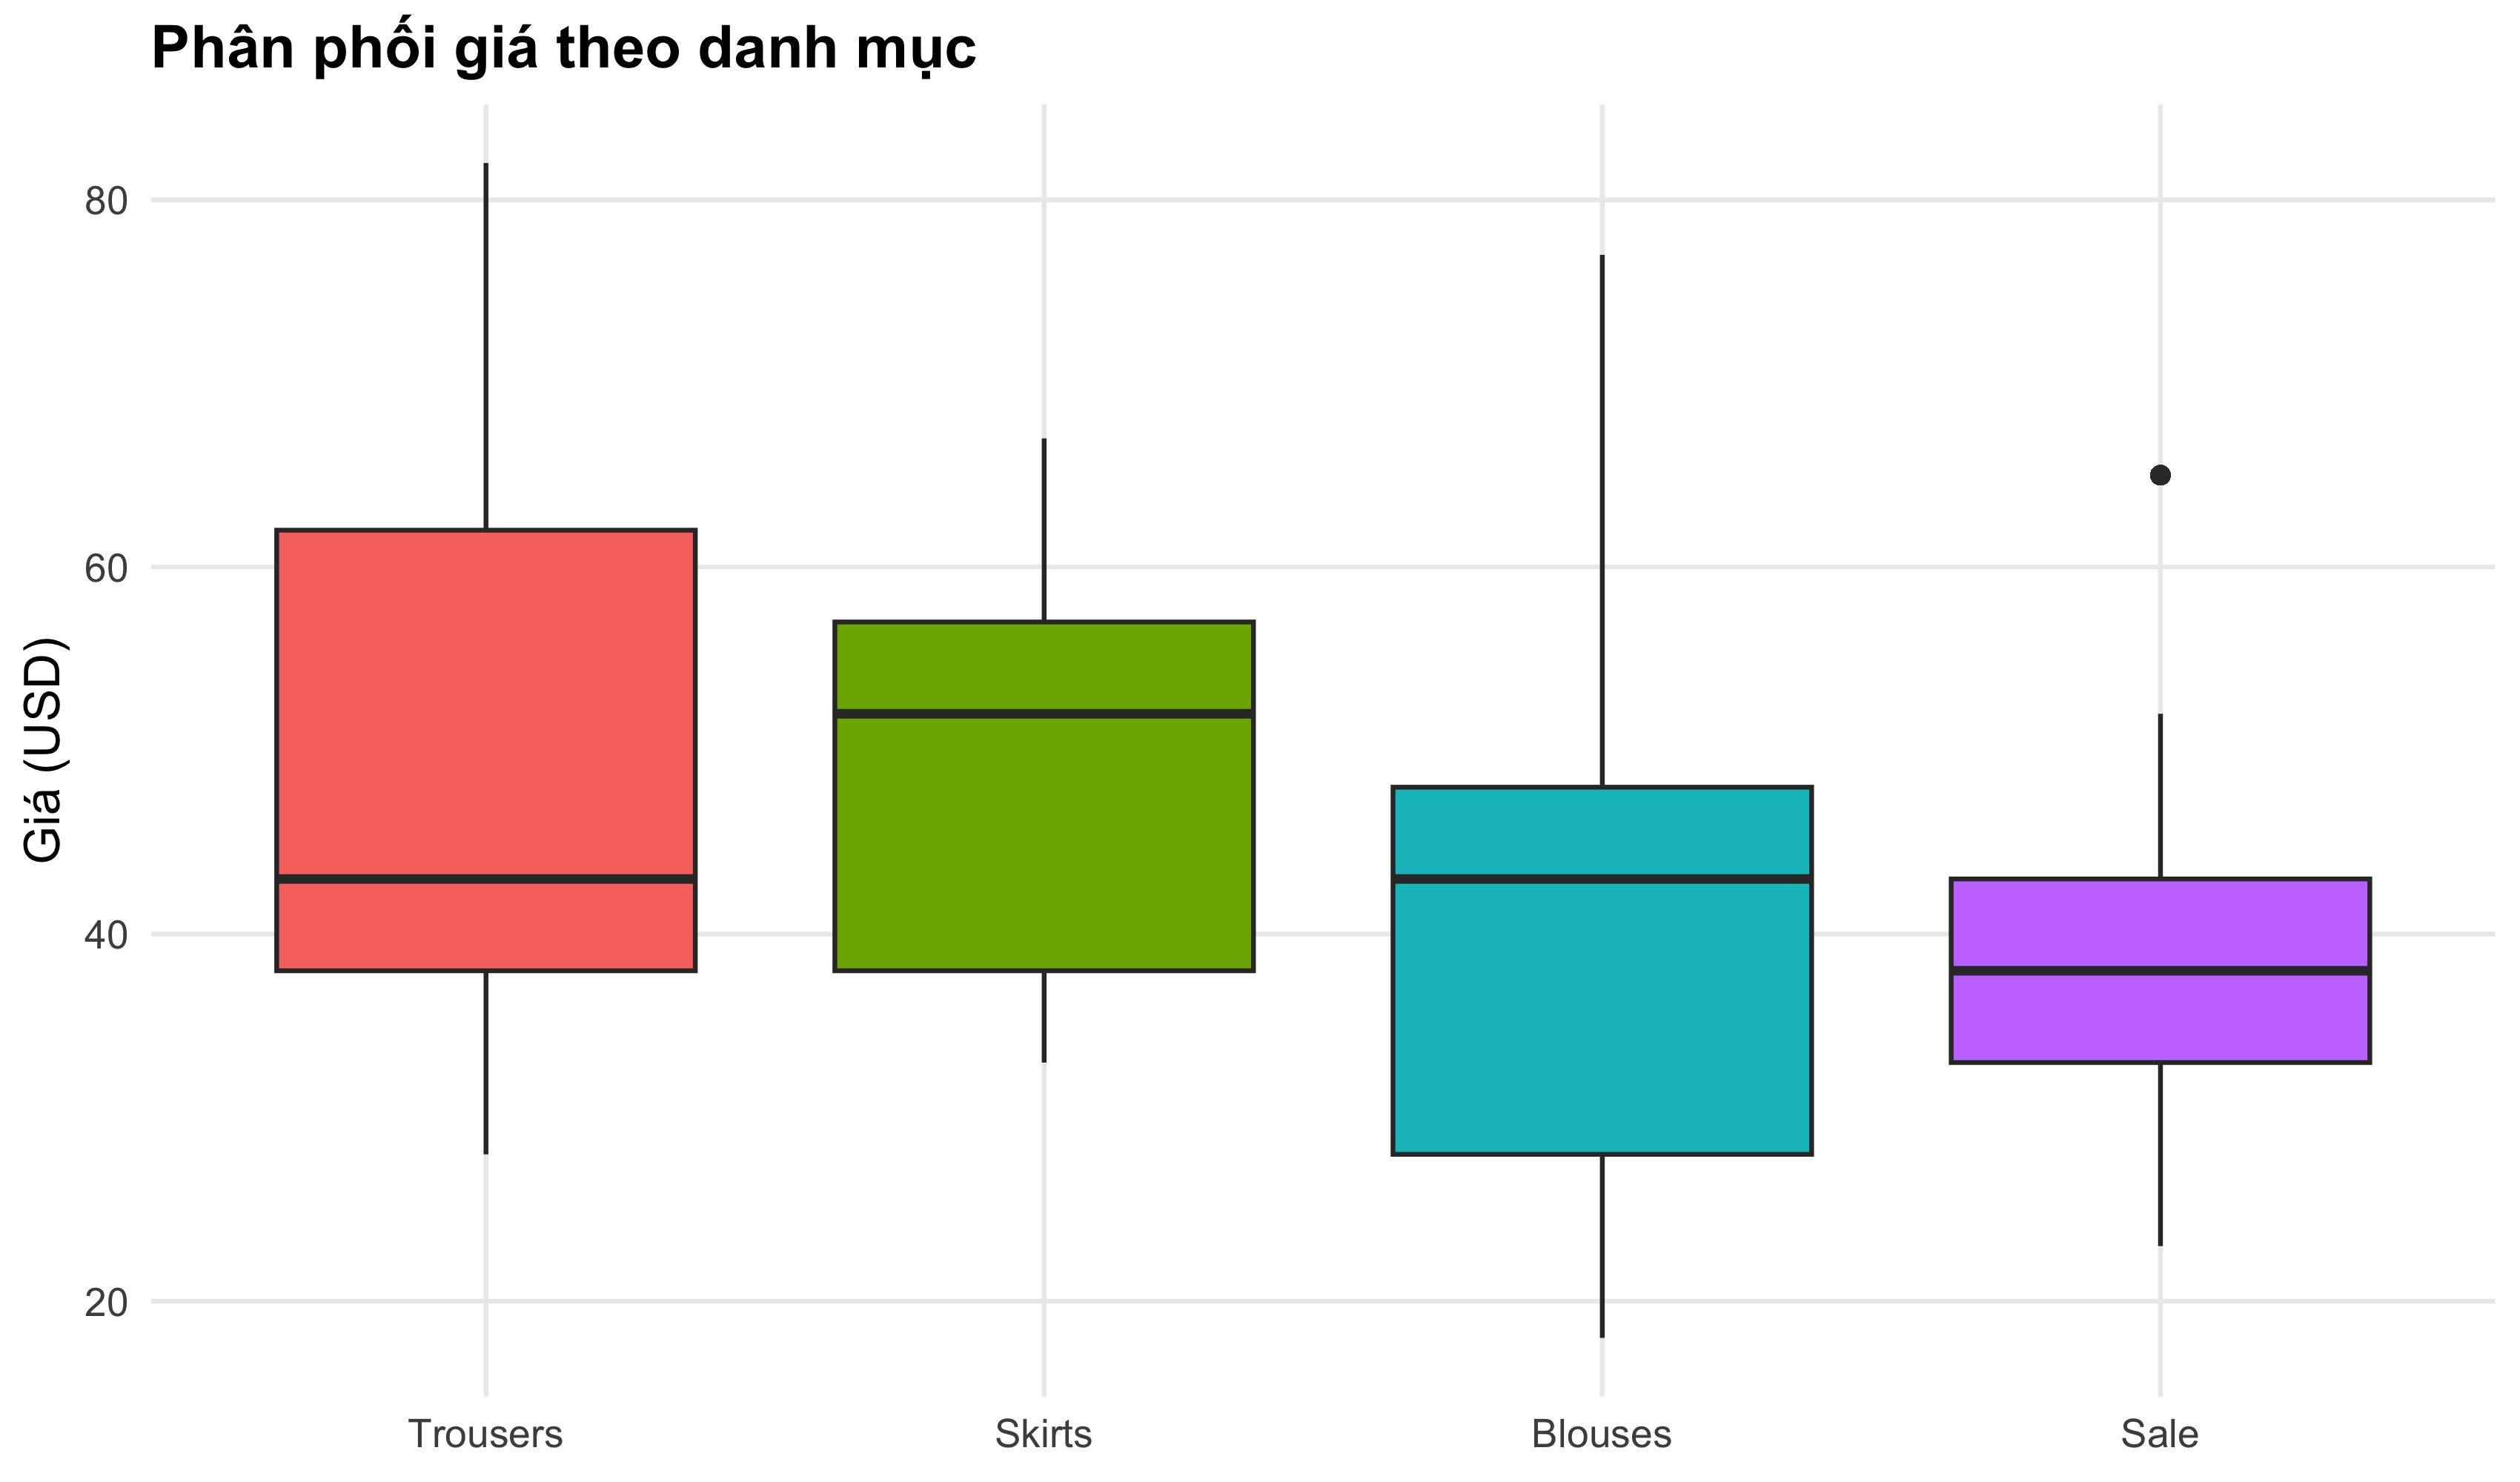
\includegraphics[width=0.85\textwidth]{img/fig-eda-price-category.png}
\caption{Phân phối giá theo danh mục sản phẩm}
\label{fig:eda-price-category}
\end{figure}

Hình~\ref{fig:eda-price-category} cho thấy mặt bằng giá khác biệt rõ giữa bốn
danh mục. Vì biến \texttt{price\_above\_avg} được xác định theo trung bình của
\emph{chính danh mục đó}, mọi phân tích so sánh hai nhóm giá bắt buộc phải kiểm
soát \texttt{category}, và không được xem nhóm giá là một treatment được ngẫu
nhiên hóa.

\begin{figure}[H]
\centering
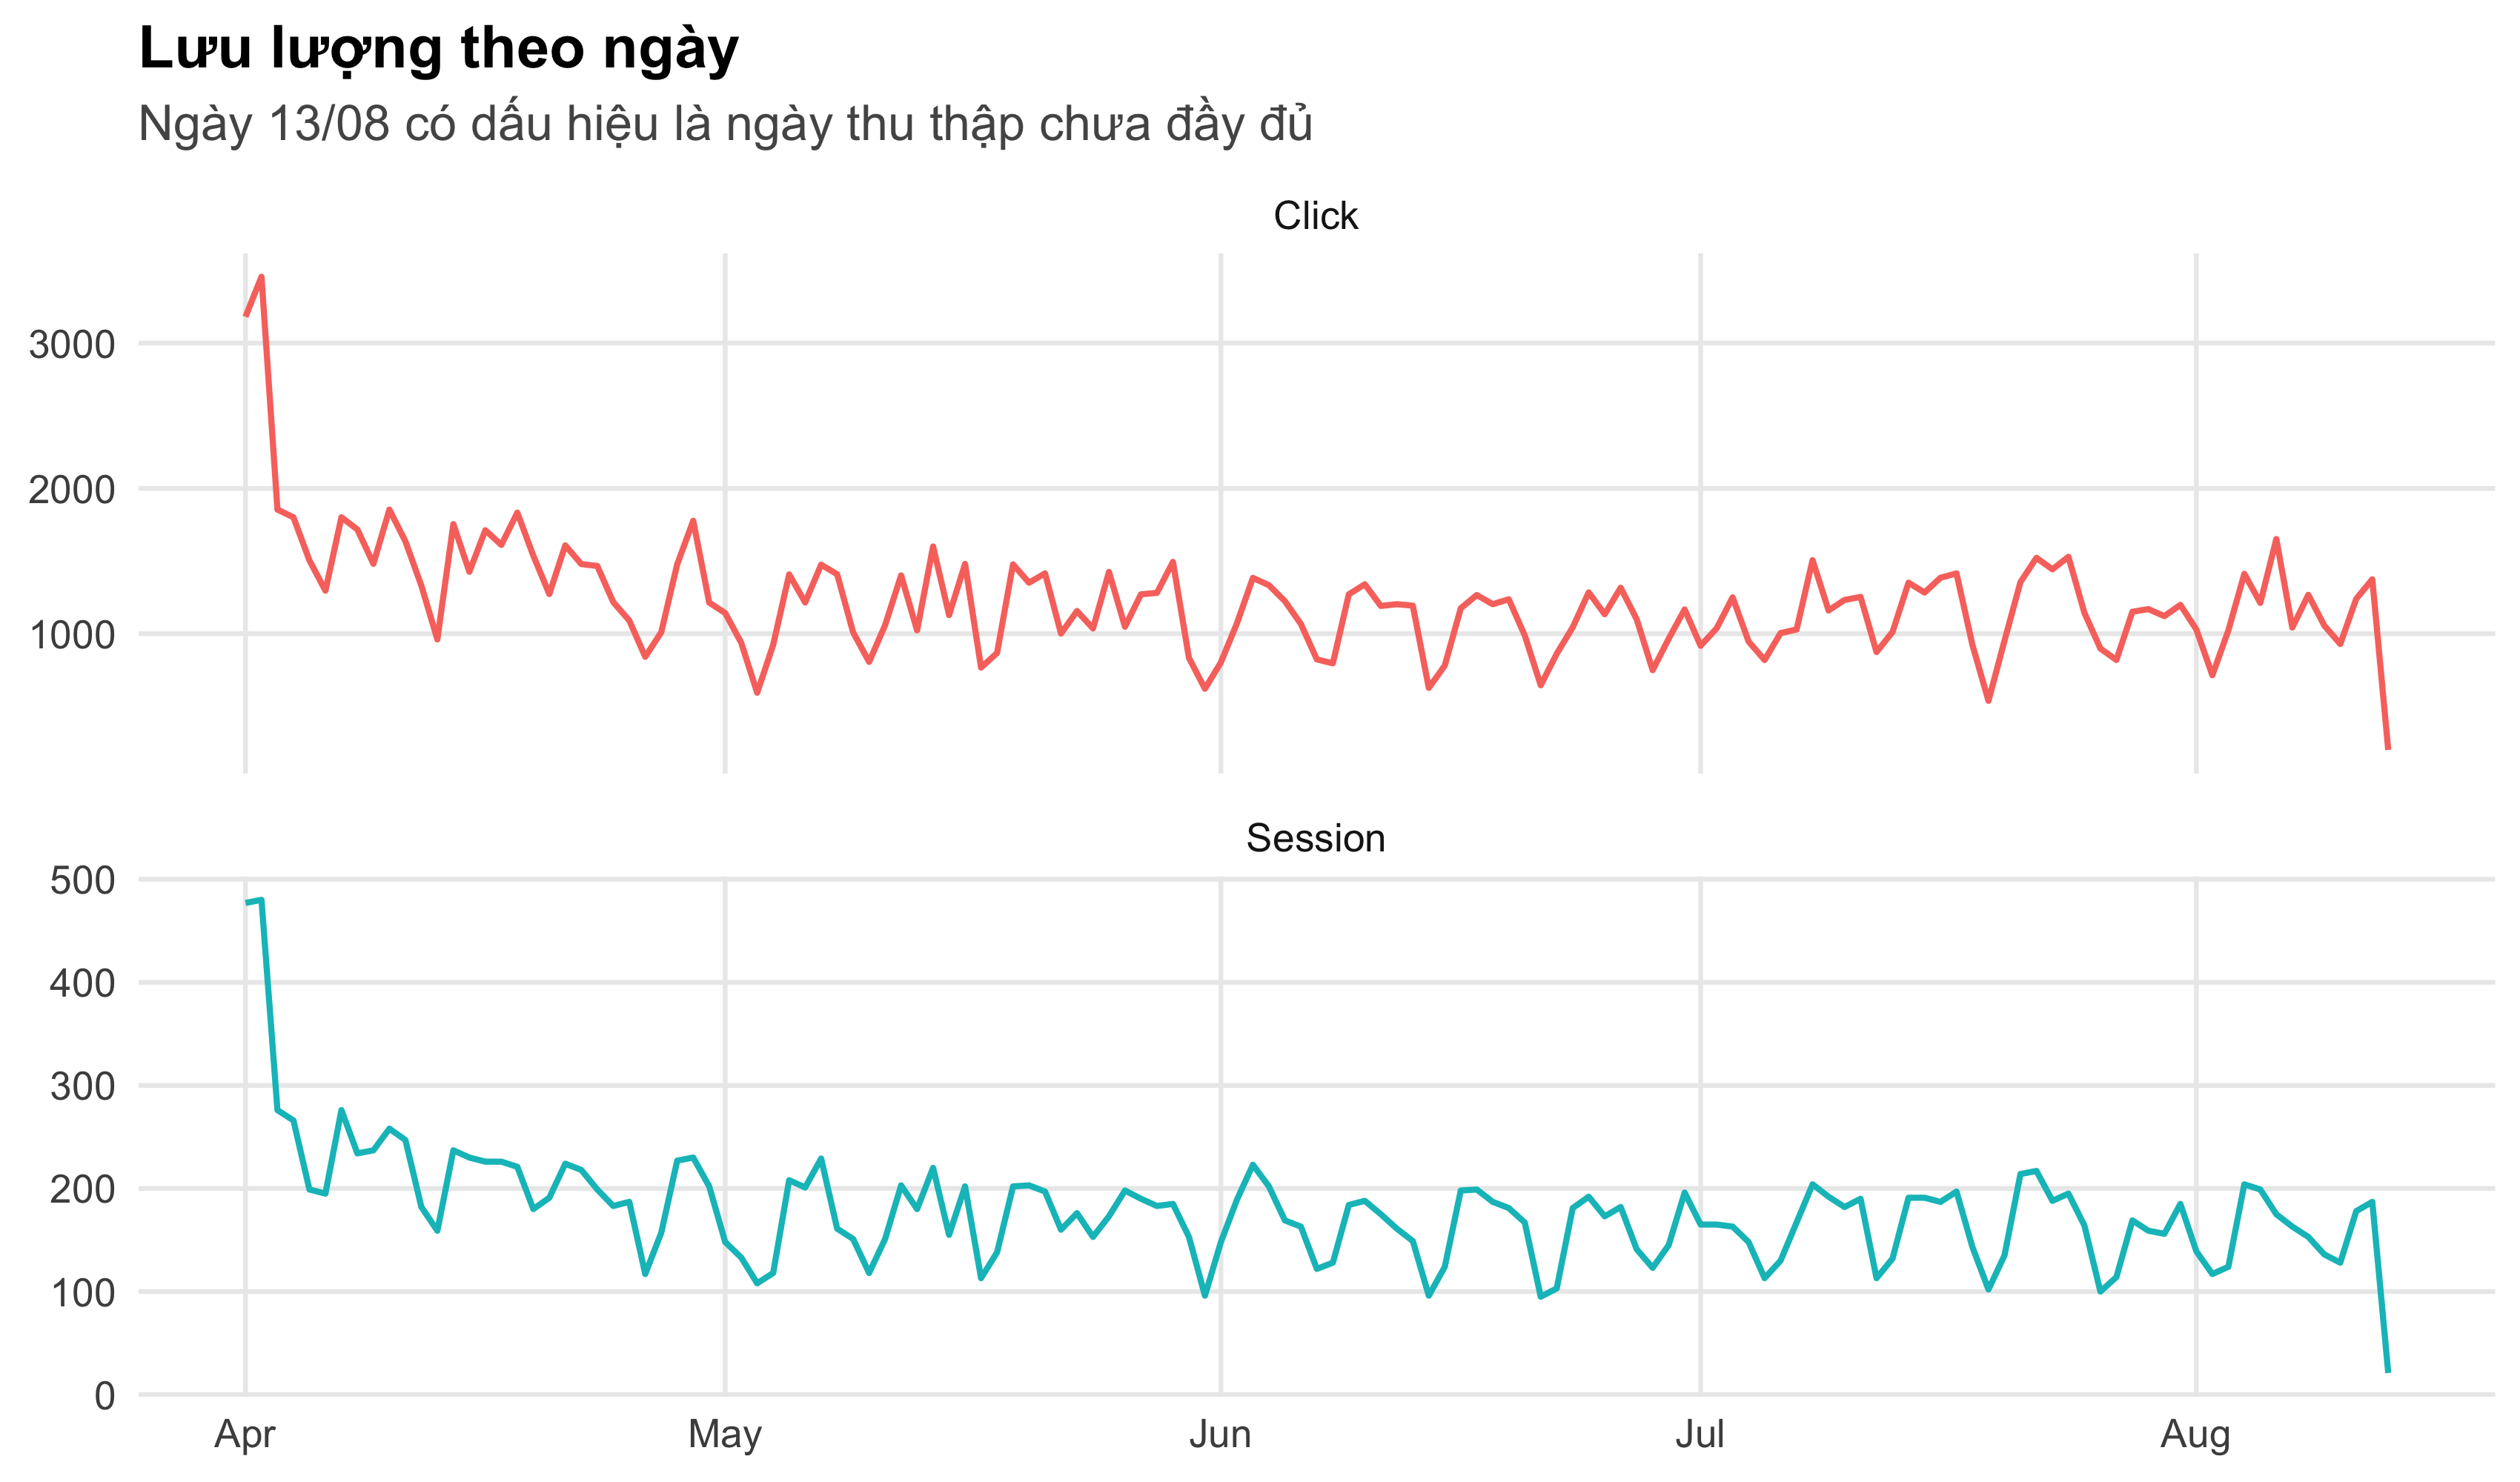
\includegraphics[width=\textwidth]{img/fig-eda-time.png}
\caption{Lưu lượng click và số session theo ngày}
\label{fig:eda-time}
\end{figure}

Chuỗi thời gian ở Hình~\ref{fig:eda-time} cho thấy lưu lượng biến động rõ theo
ngày và theo tuần, củng cố quyết định chia dữ liệu theo thời gian thay vì ngẫu
nhiên. Điểm sụt mạnh ở cuối chuỗi ứng với ngày 13/08 chỉ có 200 click, dấu hiệu
của một ngày thu thập dở dang chứ không phải bằng chứng về suy giảm lưu lượng
thực sự.

Nhóm cố ý \emph{không} trình bày ma trận tương quan Pearson cho toàn bộ các cột,
vì phần lớn biến trong bộ dữ liệu là mã factor (country, colour, location,
page\ldots); hệ số tương quan tính trên các mã số này không có ý nghĩa thống kê.
Quan hệ giữa các biến phân loại và \texttt{Exit} được đánh giá trực tiếp bằng các
mô hình ở Phần~\ref{sec:results}.

%\newpage
% Nội dung phần 3: Kết quả phân tích và mô hình hóa.
% Theo yêu cầu đề bài, phần này chỉ trình bày bảng kết quả, biểu đồ và diễn giải;
% toàn bộ mã R nằm trong file de_xuat_phan_tich_clickstream.Rmd.

\section{Kết quả phân tích và mô hình hóa}
\label{sec:results}

\subsection{Kết quả so sánh hai nhóm giá dạng A/B}
\label{subsec:ab}

Phân tích chính được thực hiện trên tập validation tháng 7 (35.231 click của
5.071 session). Nhóm A gồm các click vào sản phẩm \emph{không} có giá cao hơn
trung bình danh mục; nhóm B gồm các click vào sản phẩm có giá cao hơn trung bình
danh mục.

\subsubsection{Kết quả kiểm định}

\begin{table}[H]
\centering
\caption{Tỷ lệ Exit theo nhóm giá trên tập validation tháng 7}
\label{tab:ab-rate}
\small
\begin{tabular}{lrrrrl}
\toprule
\textbf{Nhóm} & \textbf{Click} & \textbf{Session} & \textbf{Exit}
& \textbf{Tỷ lệ Exit} & \textbf{CI 95\% (Wilson)} \\
\midrule
A: Không cao hơn TB & 16.879 & 4.147 & 2.325 & 13,77\% & 13,26\% -- 14,30\% \\
B: Cao hơn TB       & 18.352 & 4.249 & 2.746 & 14,96\% & 14,45\% -- 15,49\% \\
\bottomrule
\end{tabular}
\end{table}

Một session có thể xem sản phẩm thuộc cả hai nhóm giá, nên tổng số session ở hai
hàng của Bảng~\ref{tab:ab-rate} lớn hơn 5.071 và không được cộng lại.

\begin{table}[H]
\centering
\caption{Tổng hợp các kiểm định so sánh hai nhóm giá (tháng 7)}
\label{tab:ab-test}
\small
\begin{tabular}{>{\raggedright\arraybackslash}p{0.30\textwidth}rll}
\toprule
\textbf{Đại lượng} & \textbf{Ước lượng} & \textbf{CI 95\%} & \textbf{p-value} \\
\midrule
Chênh lệch thô B $-$ A (điểm \%)      & 1,19  & 0,46 -- 1,93 (cluster bootstrap) & --- \\
Kiểm định hai tỷ lệ ($\chi^2$, df = 1) & 10,08 & ---                              & 0,002 \\
Adjusted odds ratio (B so với A)       & 1,071 & 1,002 -- 1,144 (robust)          & 0,043 \\
Adjusted risk difference (điểm \%)     & 0,82  & 0,03 -- 1,62 (robust)            & --- \\
Tương tác nhóm giá $\times$ Category   & ---   & ---                              & 0,051 \\
\bottomrule
\end{tabular}
\end{table}

Ở mức ý nghĩa 5\%, cả kiểm định hai tỷ lệ thô ($p = 0{,}002$) lẫn adjusted odds
ratio với sai số chuẩn cluster-robust theo session ($p = 0{,}043$) đều cho phép
\textbf{bác bỏ $H_0$}. Tuy nhiên độ lớn hiệu ứng rất khiêm tốn: sau khi điều
chỉnh tiến trình session, thời gian, country và toàn bộ đặc điểm sản phẩm, chênh
lệch xác suất chuẩn hóa chỉ còn 0,82 điểm phần trăm, với cận dưới của khoảng tin
cậy sát 0 (0,03 điểm phần trăm). Nói cách khác, bằng chứng về sự \emph{tồn tại}
của khác biệt là có, nhưng khác biệt đó nhỏ và ước lượng kém chính xác.

\begin{figure}[H]
\centering
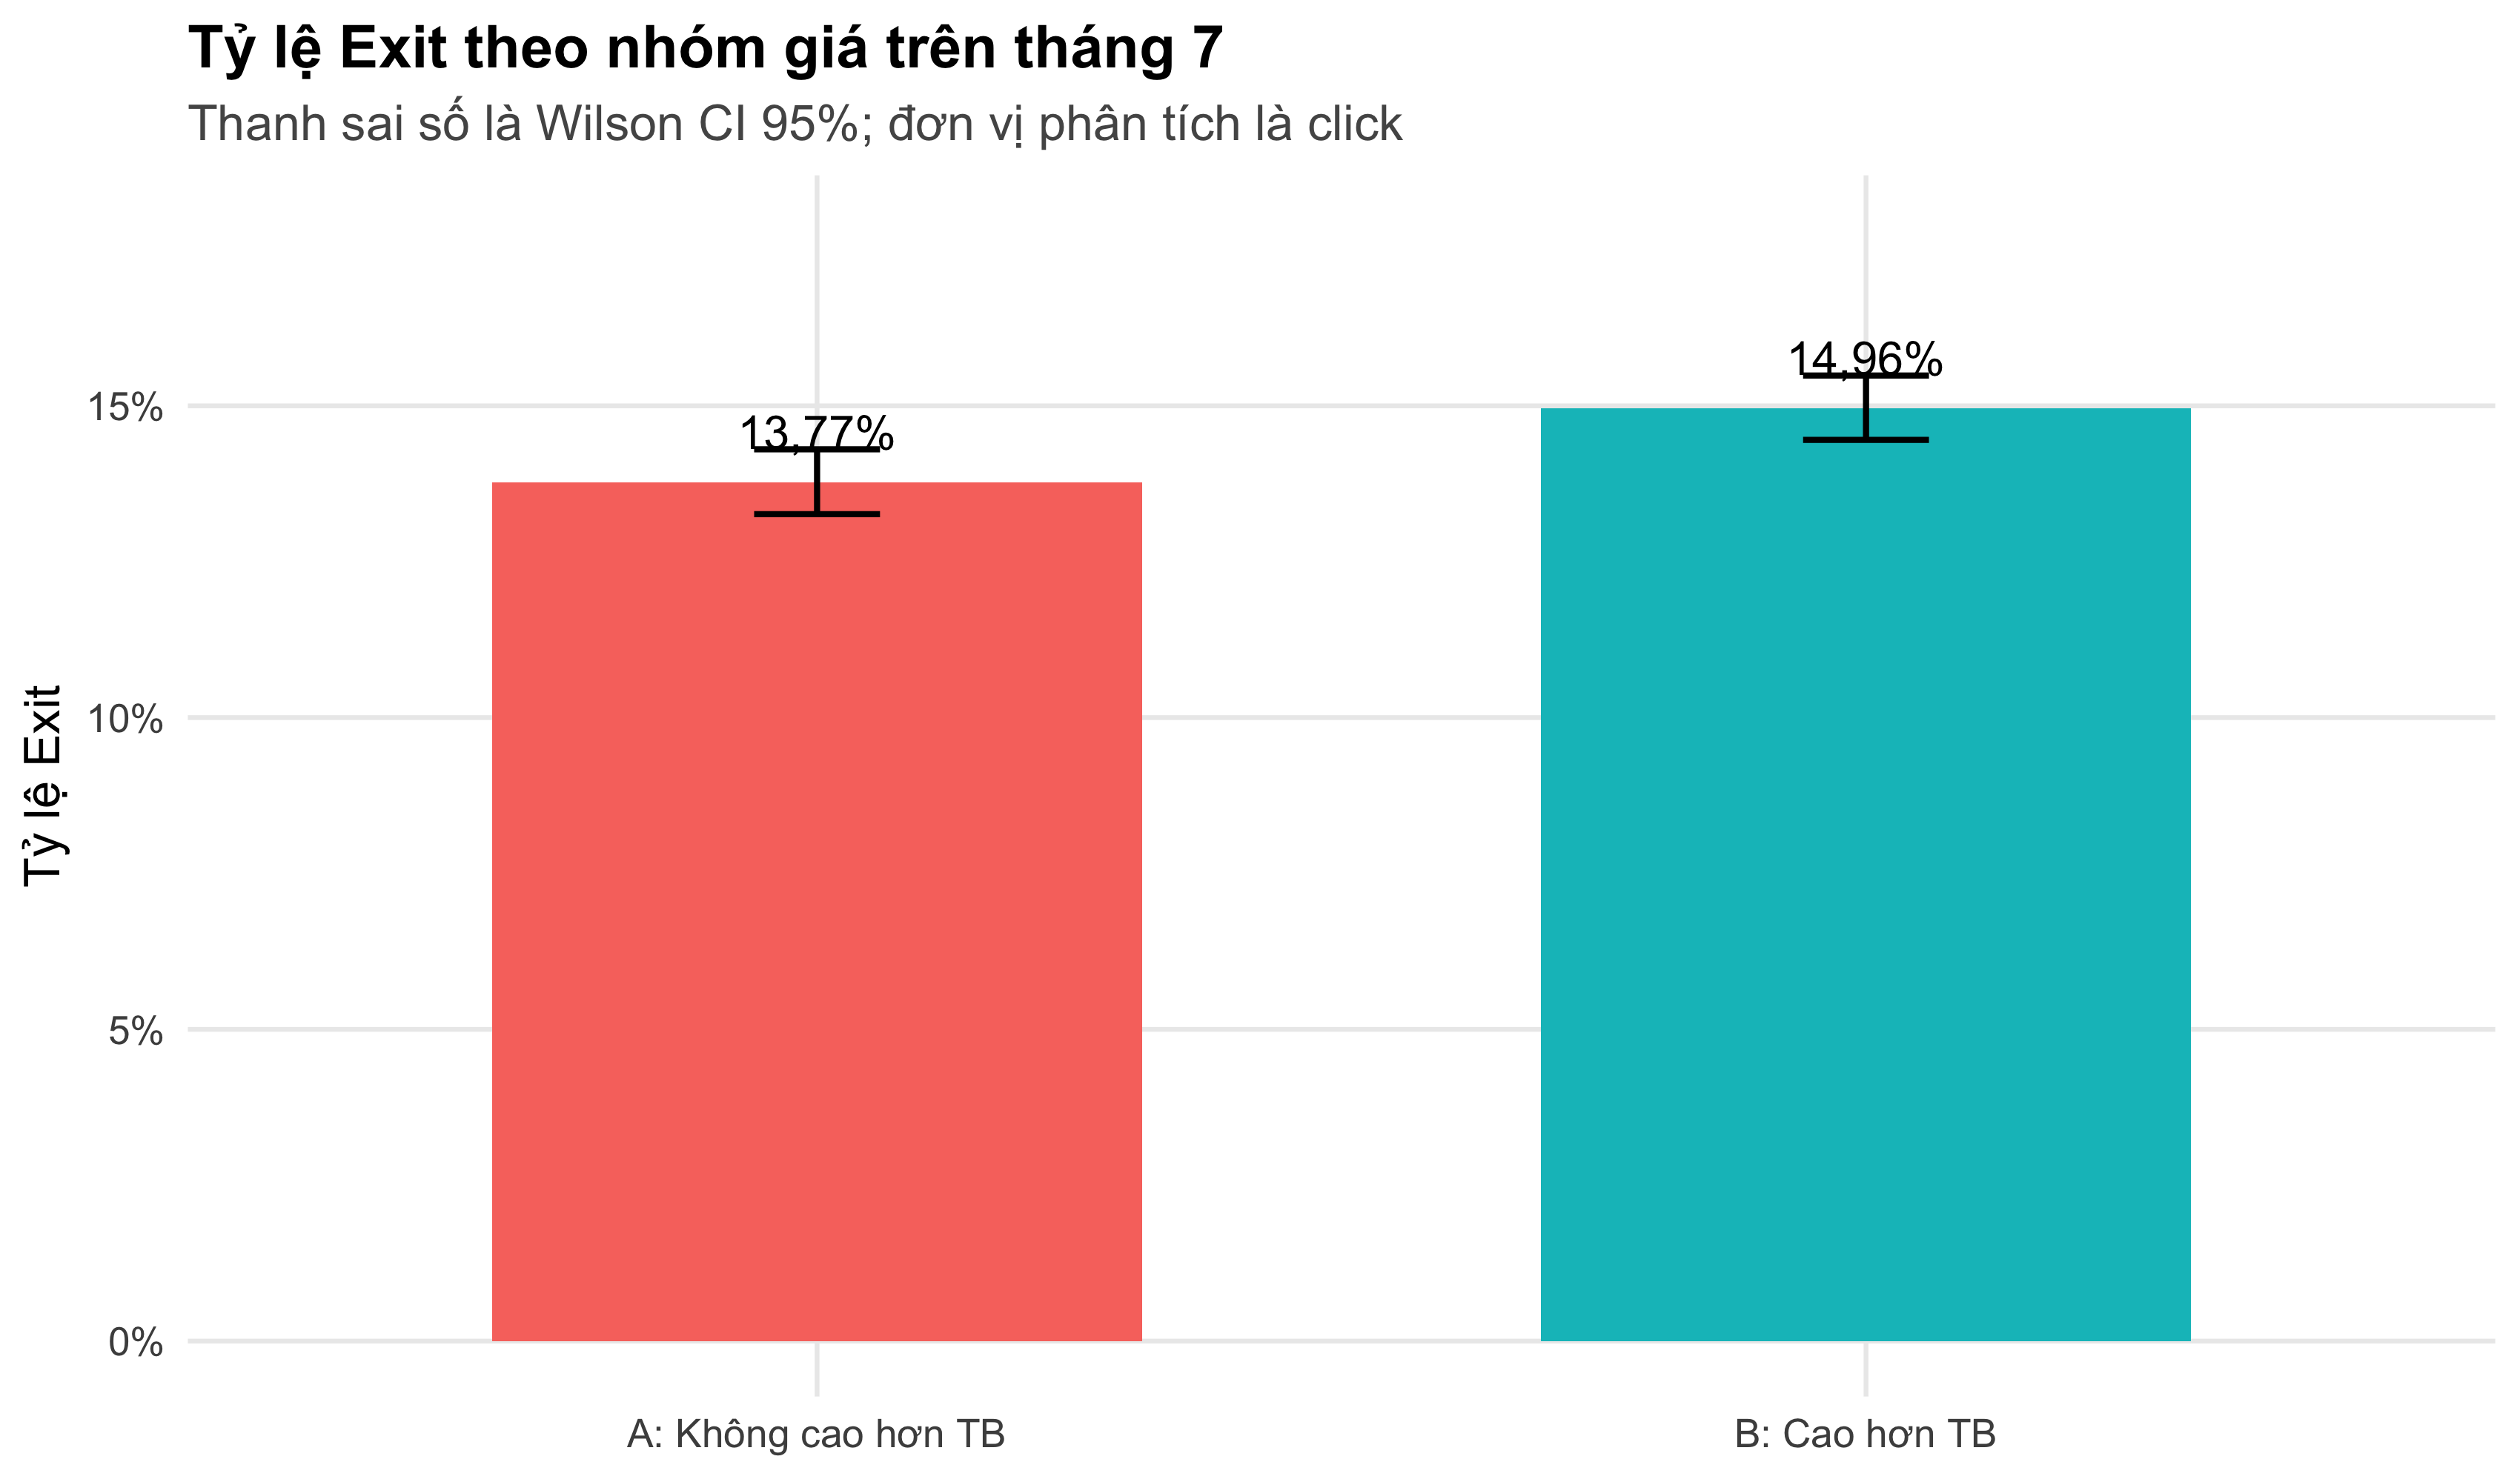
\includegraphics[width=0.8\textwidth]{img/fig-ab-exit-rate.png}
\caption{So sánh tỷ lệ Exit giữa hai nhóm giá trên tháng 7, thanh sai số là
khoảng tin cậy Wilson 95\%}
\label{fig:ab-exit-rate}
\end{figure}

\subsubsection{Kiểm tra balance giữa hai nhóm}

\begin{figure}[H]
\centering
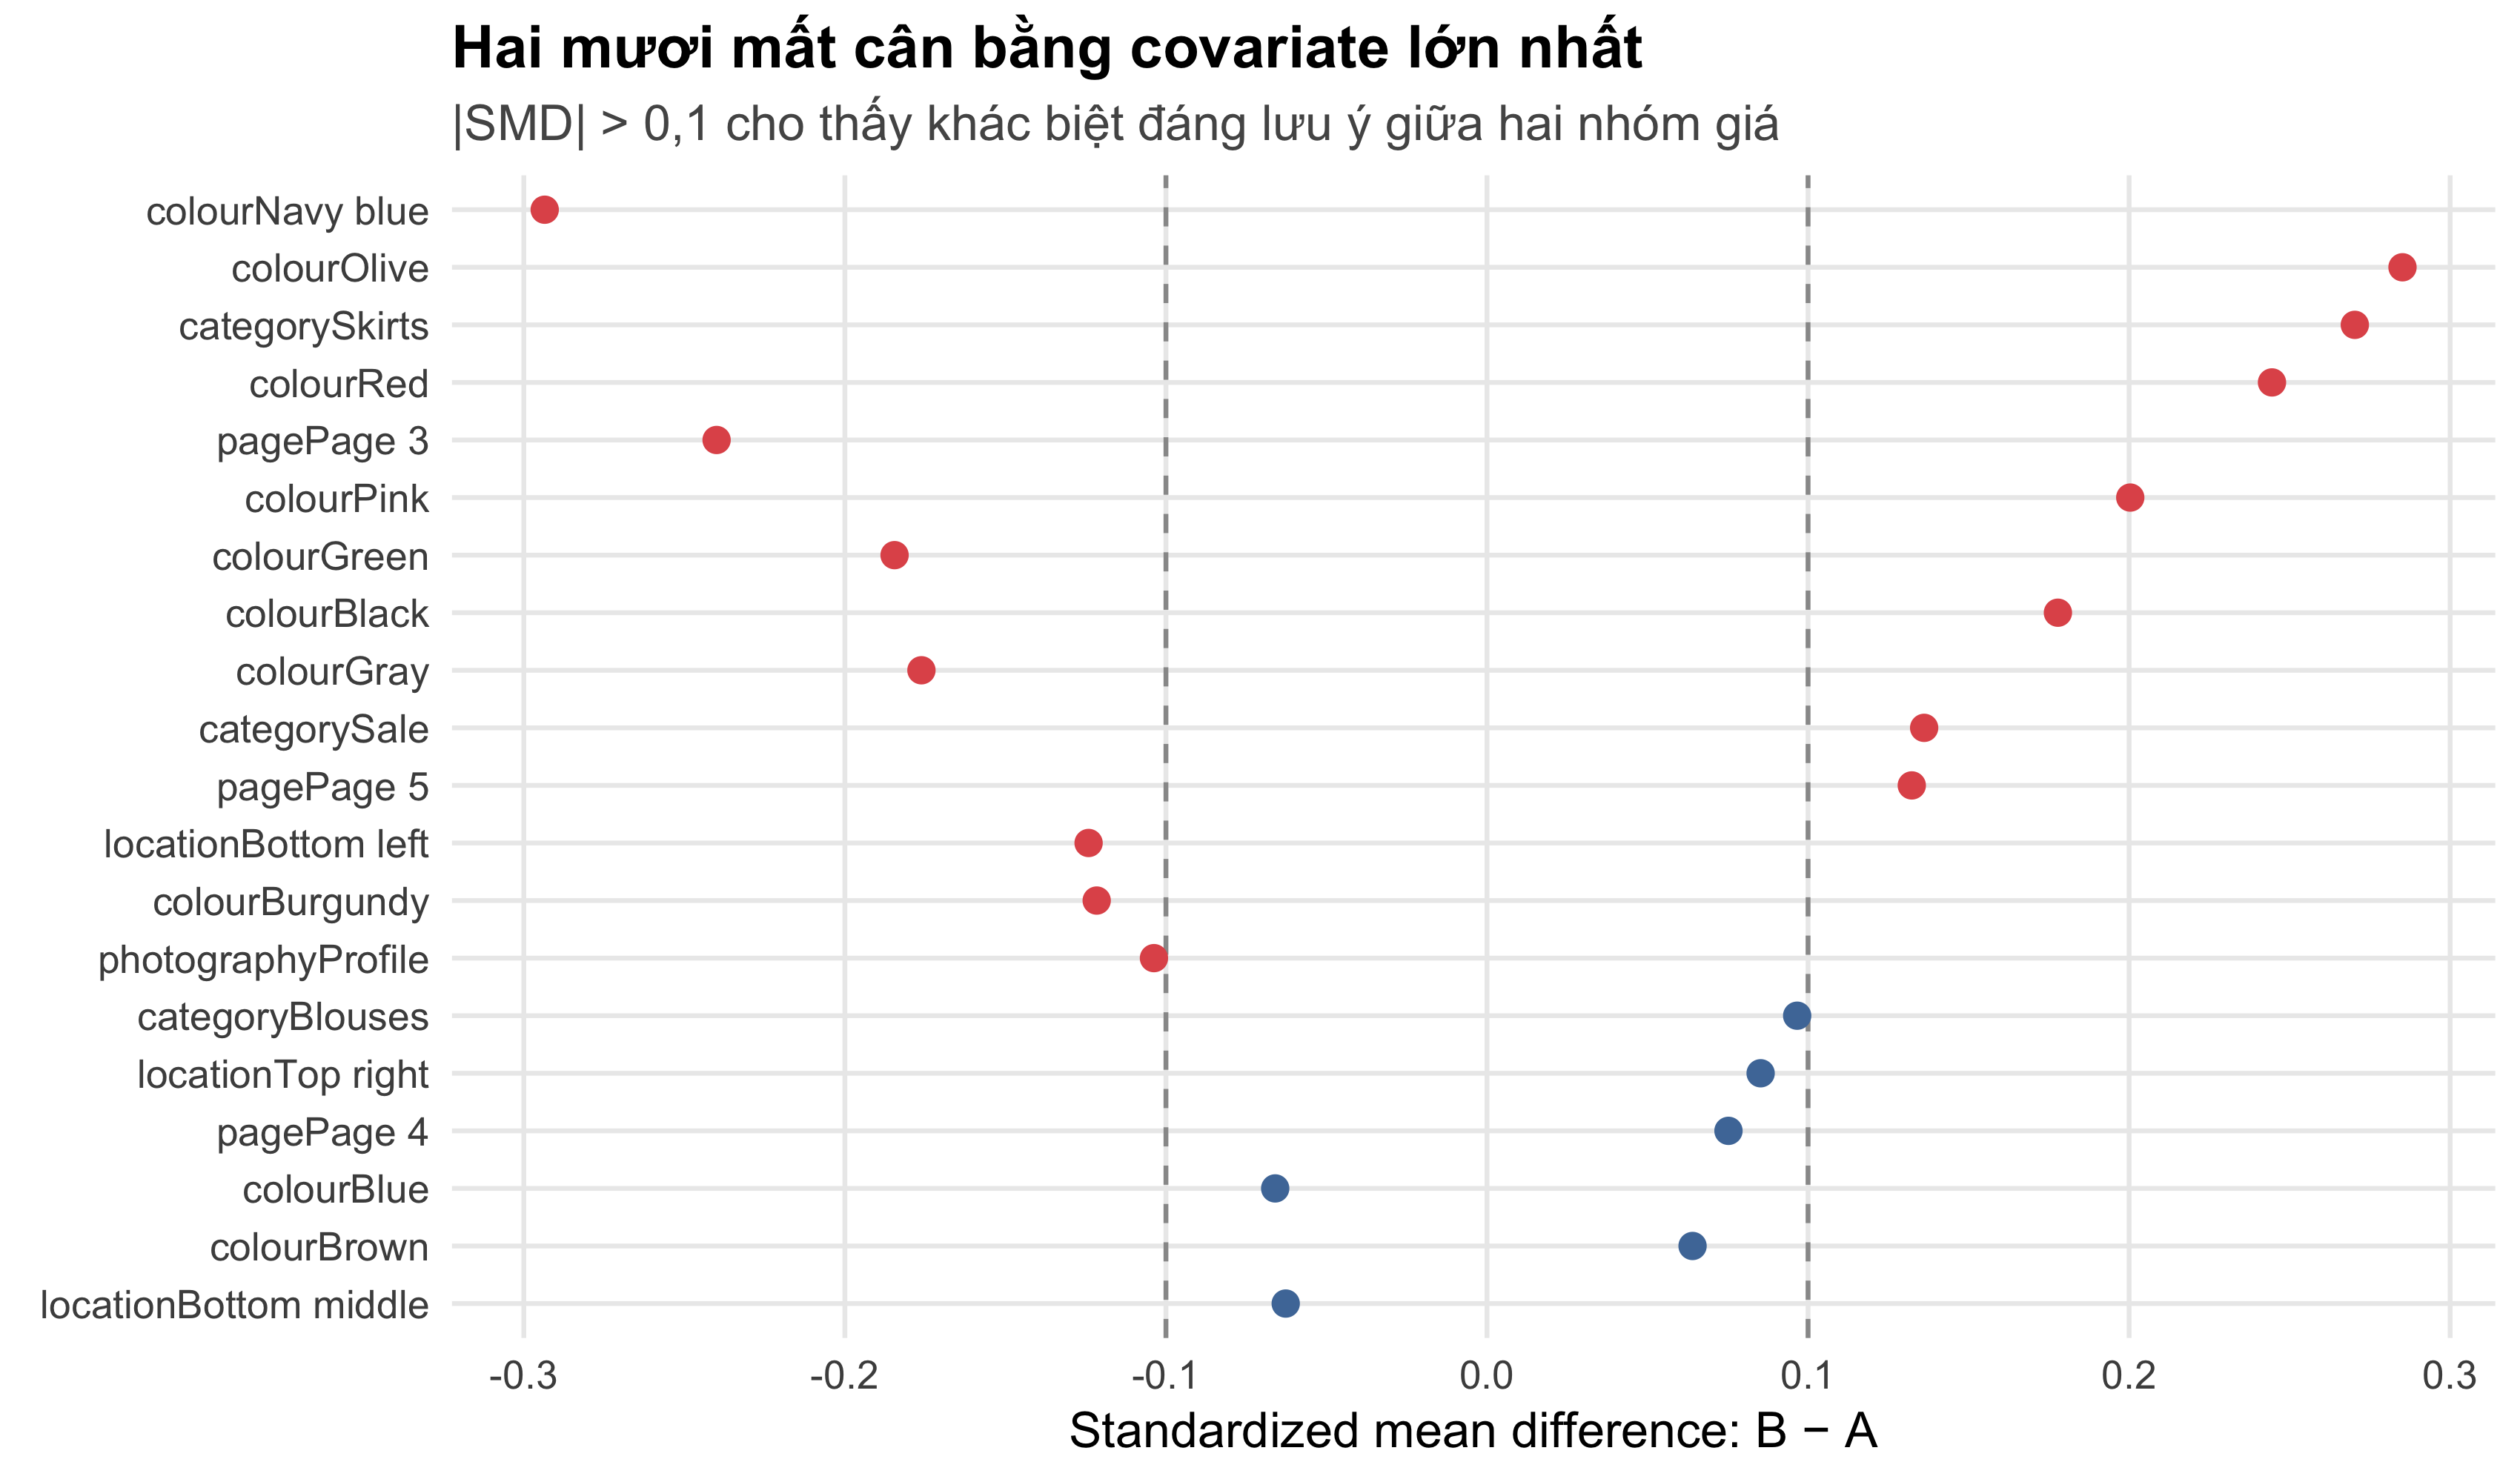
\includegraphics[width=\textwidth]{img/fig-ab-balance.png}
\caption{Hai mươi covariate mất cân bằng nhất giữa hai nhóm giá}
\label{fig:ab-balance}
\end{figure}

Hình~\ref{fig:ab-balance} là bằng chứng trực tiếp cho thấy hai nhóm \emph{không}
tương đương như trong một thí nghiệm ngẫu nhiên: nhiều covariate có
$|\text{SMD}| > 0{,}1$. Đây là lý do báo cáo ưu tiên adjusted risk difference và
suy luận robust thay vì chênh lệch thô. Dù vậy, việc điều chỉnh chỉ xử lý được
các yếu tố \emph{đã quan sát}; residual confounding vẫn có thể tồn tại.

\subsubsection{Dị biệt hiệu ứng theo danh mục}

\begin{table}[H]
\centering
\caption{Adjusted risk difference của nhóm giá theo từng danh mục (tháng 7)}
\label{tab:ab-category}
\small
\begin{tabular}{lrrll}
\toprule
\textbf{Category} & \textbf{N} & \textbf{Adjusted RD (điểm \%)}
& \textbf{CI 95\%} & \textbf{p-value (Holm)} \\
\midrule
Trousers & 10.871 & 2,32          & 0,86 -- 3,78            & 0,008 \\
Skirts   & 7.382  & 0,69          & $-$1,25 -- 2,62         & 1,000 \\
Blouses  & 7.858  & 0,72          & $-$0,88 -- 2,33         & 1,000 \\
Sale     & 9.120  & $-$0,66       & $-$2,17 -- 0,85         & 1,000 \\
\bottomrule
\end{tabular}
\end{table}

\begin{figure}[H]
\centering
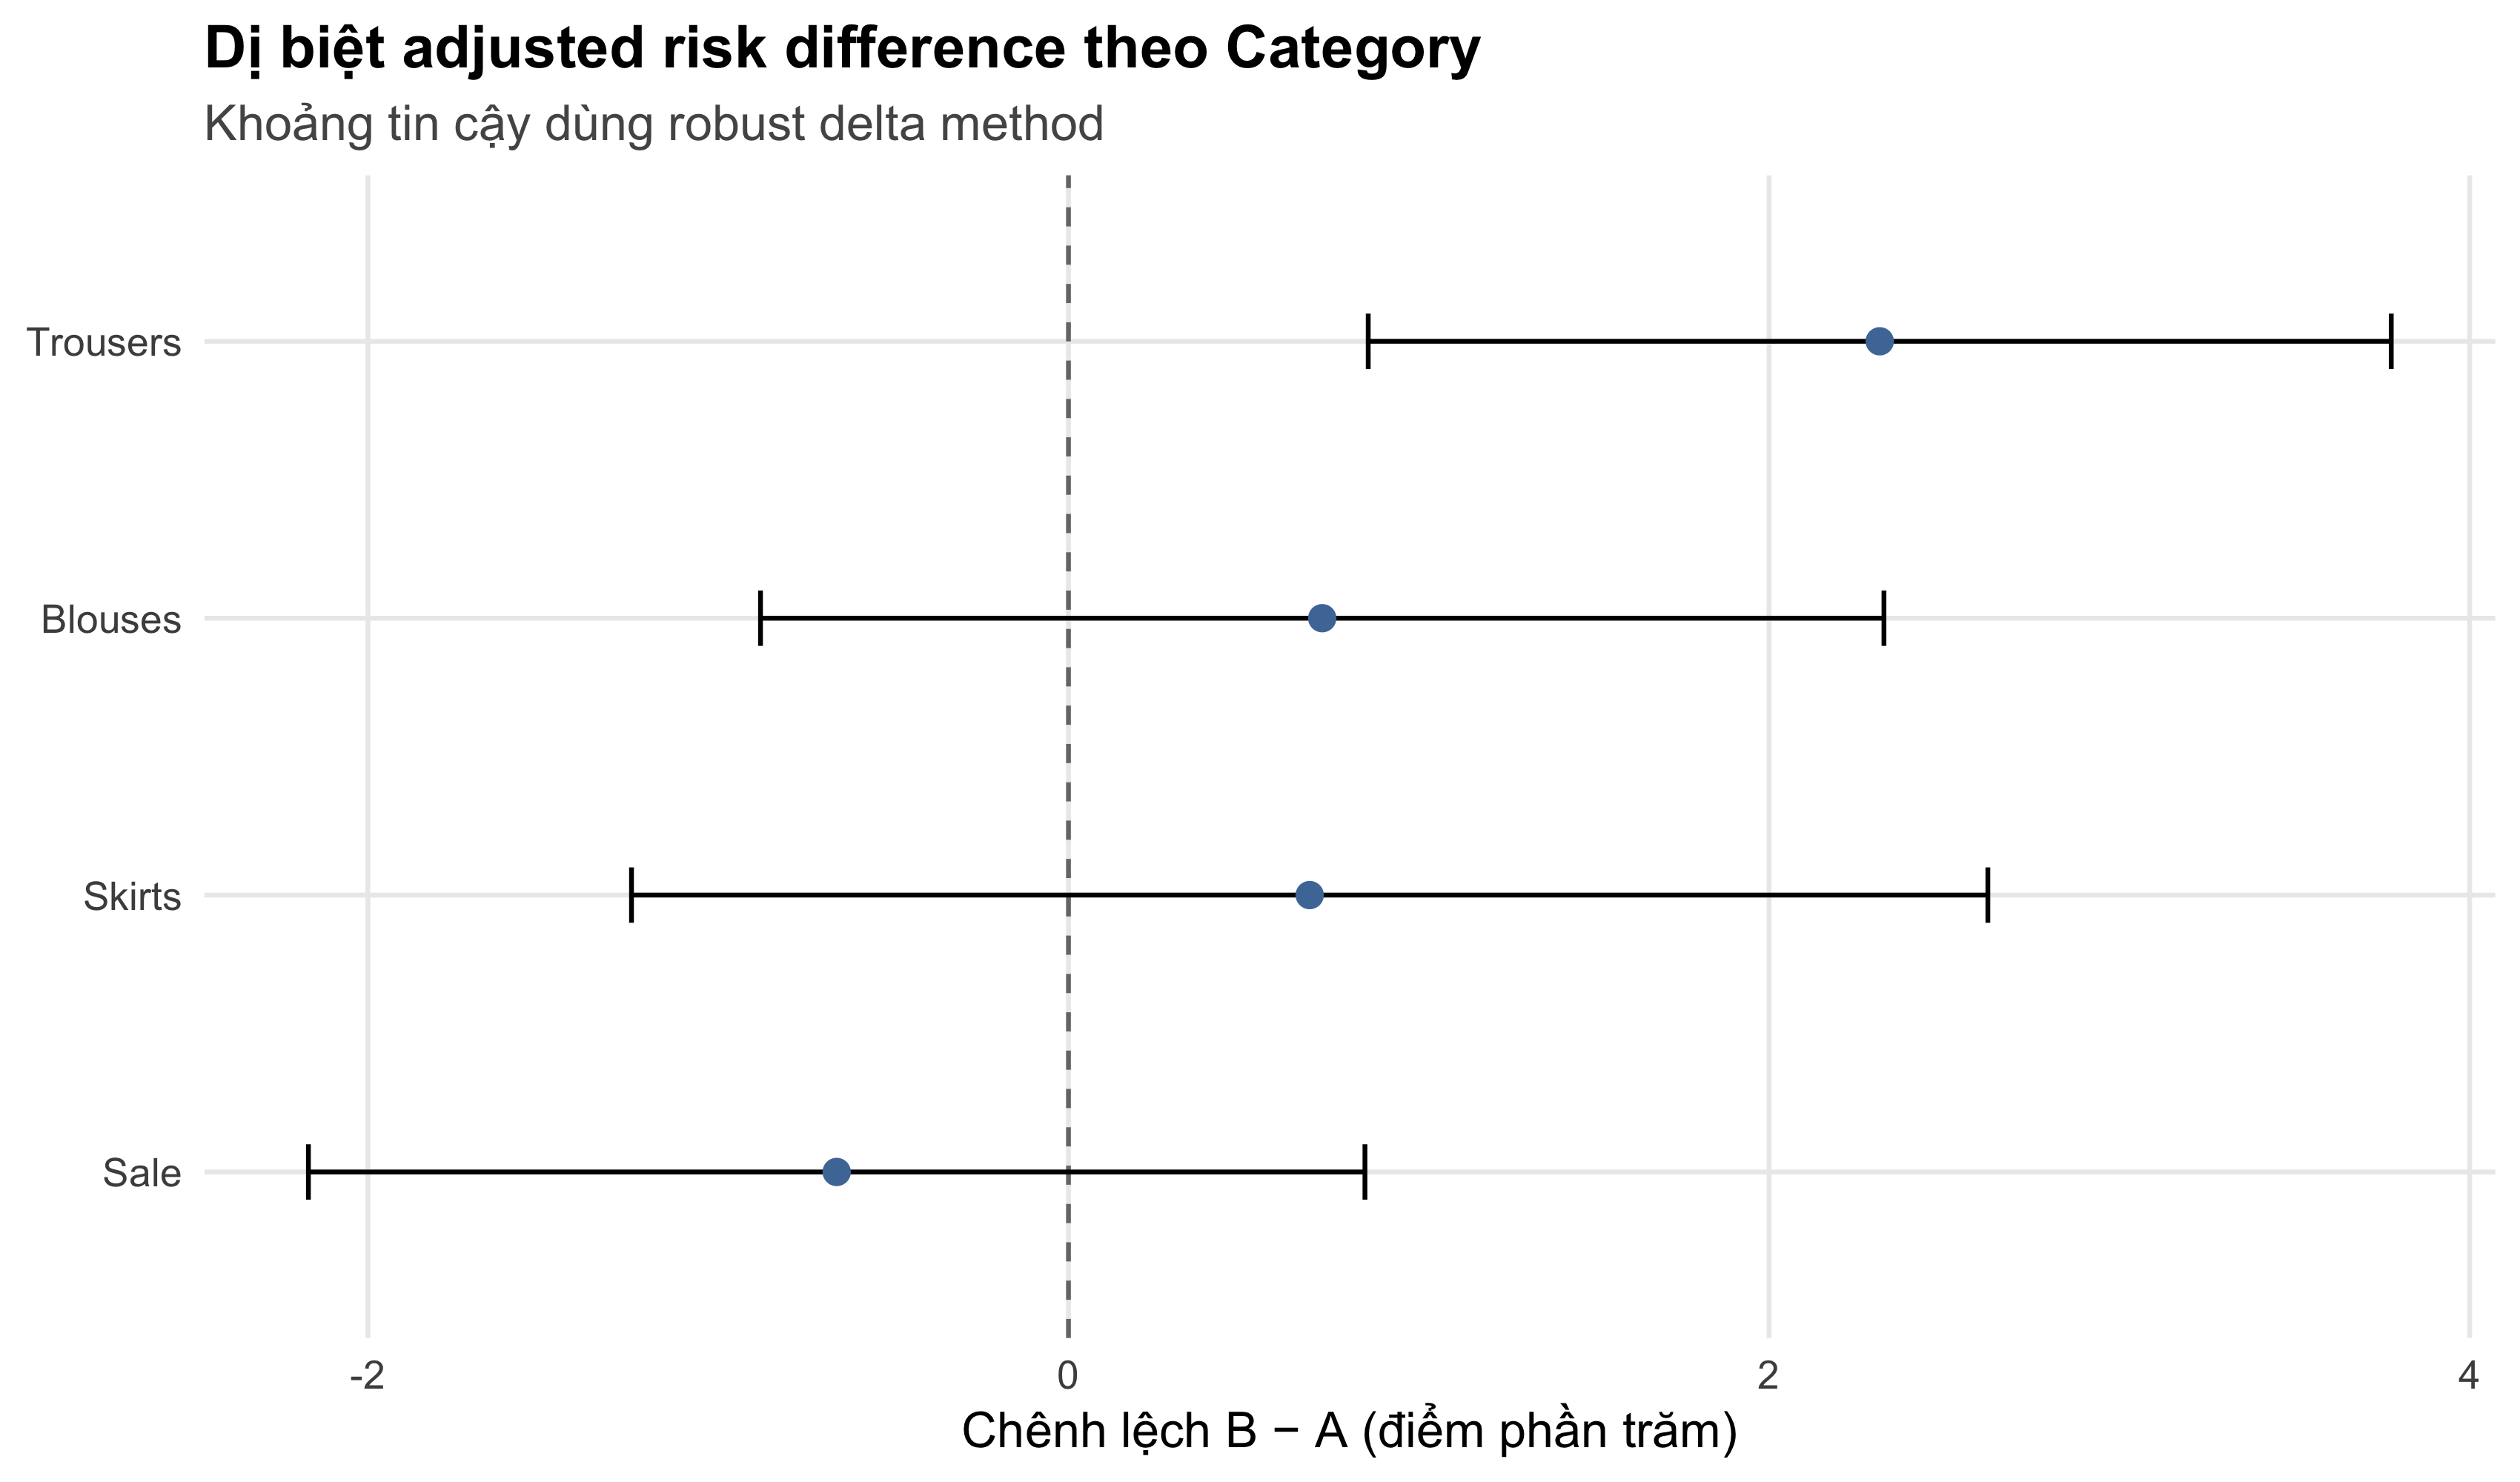
\includegraphics[width=0.85\textwidth]{img/fig-ab-forest.png}
\caption{Forest plot adjusted risk difference của nhóm giá theo danh mục}
\label{fig:ab-forest}
\end{figure}

Kiểm định Wald robust cho toàn bộ nhóm tương tác \texttt{price group} $\times$
\texttt{Category} cho $p = 0{,}051$, tức nằm ngay ranh giới 5\%. Sau hiệu chỉnh
Holm, chỉ riêng danh mục Trousers còn khác biệt có ý nghĩa (2,32 điểm phần trăm,
$p = 0{,}008$); ba danh mục còn lại đều có khoảng tin cậy chứa 0, và Sale thậm
chí có dấu ngược lại. Điều này cho thấy hiệu ứng gộp ở Bảng~\ref{tab:ab-test}
không đại diện đồng đều cho mọi danh mục.

\subsubsection{Độ ổn định theo thời gian}

\begin{table}[H]
\centering
\caption{Độ ổn định theo thời gian của khác biệt giữa hai nhóm giá}
\label{tab:ab-temporal}
\small
\begin{tabular}{lrrll}
\toprule
\textbf{Giai đoạn} & \textbf{Chênh lệch B $-$ A (điểm \%)}
& \textbf{OR điều chỉnh} & \textbf{CI 95\%} & \textbf{p-value} \\
\midrule
Train: tháng 4--6             & 0,78 & 1,066 & 1,032 -- 1,102 & $< 0{,}001$ \\
Phân tích chính: tháng 7      & 1,19 & 1,108 & 1,044 -- 1,175 & $< 0{,}001$ \\
Kiểm tra thời gian: 01--12/08 & 1,36 & 1,125 & 1,021 -- 1,240 & 0,017 \\
\bottomrule
\end{tabular}
\end{table}

Để so sánh nhất quán giữa ba giai đoạn, odds ratio trong
Bảng~\ref{tab:ab-temporal} chỉ điều chỉnh $\log_2(\texttt{order})$, thời gian và
country; vì vậy nó lớn hơn odds ratio 1,071 của mô hình A/B chính -- mô hình đó
còn điều chỉnh thêm toàn bộ đặc điểm sản phẩm nên cho ước lượng thận trọng hơn.

Khác biệt có cùng dấu và độ lớn tương đương trong cả ba giai đoạn, cho thấy đây
là một mối liên hệ ổn định theo thời gian chứ không phải nhiễu ngẫu nhiên của
riêng tháng 7. Tuy nhiên, \texttt{price\_above\_avg} vẫn là một thuộc tính của
sản phẩm chứ không phải treatment được gán ngẫu nhiên, nên kết quả này
\textbf{không} chứng minh rằng tăng giá gây ra việc kết thúc session.

\subsection{Kết quả mô hình dự đoán: xác suất Exit theo tiến trình session}

\begin{table}[H]
\centering
\caption{Tỷ lệ Exit gộp theo khoảng Order trên tháng 7}
\label{tab:hazard}
\small
\begin{tabular}{lrrrl}
\toprule
\textbf{Khoảng Order} & \textbf{Click có nguy cơ} & \textbf{Click kết thúc}
& \textbf{Tỷ lệ Exit} & \textbf{CI 95\%} \\
\midrule
1      & 5.071 & 1.038 & 20,47\% & 19,38\% -- 21,60\% \\
2      & 4.033 & 707   & 17,53\% & 16,39\% -- 18,73\% \\
3--4   & 6.101 & 991   & 16,24\% & 15,34\% -- 17,19\% \\
5--7   & 6.043 & 875   & 14,48\% & 13,61\% -- 15,39\% \\
8--12  & 5.621 & 731   & 13,00\% & 12,15\% -- 13,91\% \\
13--20 & 4.197 & 411   & 9,79\%  & 8,93\% -- 10,73\% \\
$>$20  & 4.165 & 318   & 7,64\%  & 6,87\% -- 8,48\% \\
\bottomrule
\end{tabular}
\end{table}

Xác suất kết thúc giảm gần như đơn điệu theo tiến trình session: từ 20,47\% tại
click đầu tiên xuống 7,64\% với các click sau vị trí 20 -- tức giảm hơn một nửa.
Lưu ý mẫu số ở mỗi hàng là số click \emph{có nguy cơ} trong khoảng đó, không phải
số session ở đầu khoảng; cách tính này tránh diễn giải sai rằng mọi session sống
sót qua click 20 đều có cùng xác suất kết thúc ngay lập tức.

\begin{figure}[H]
\centering
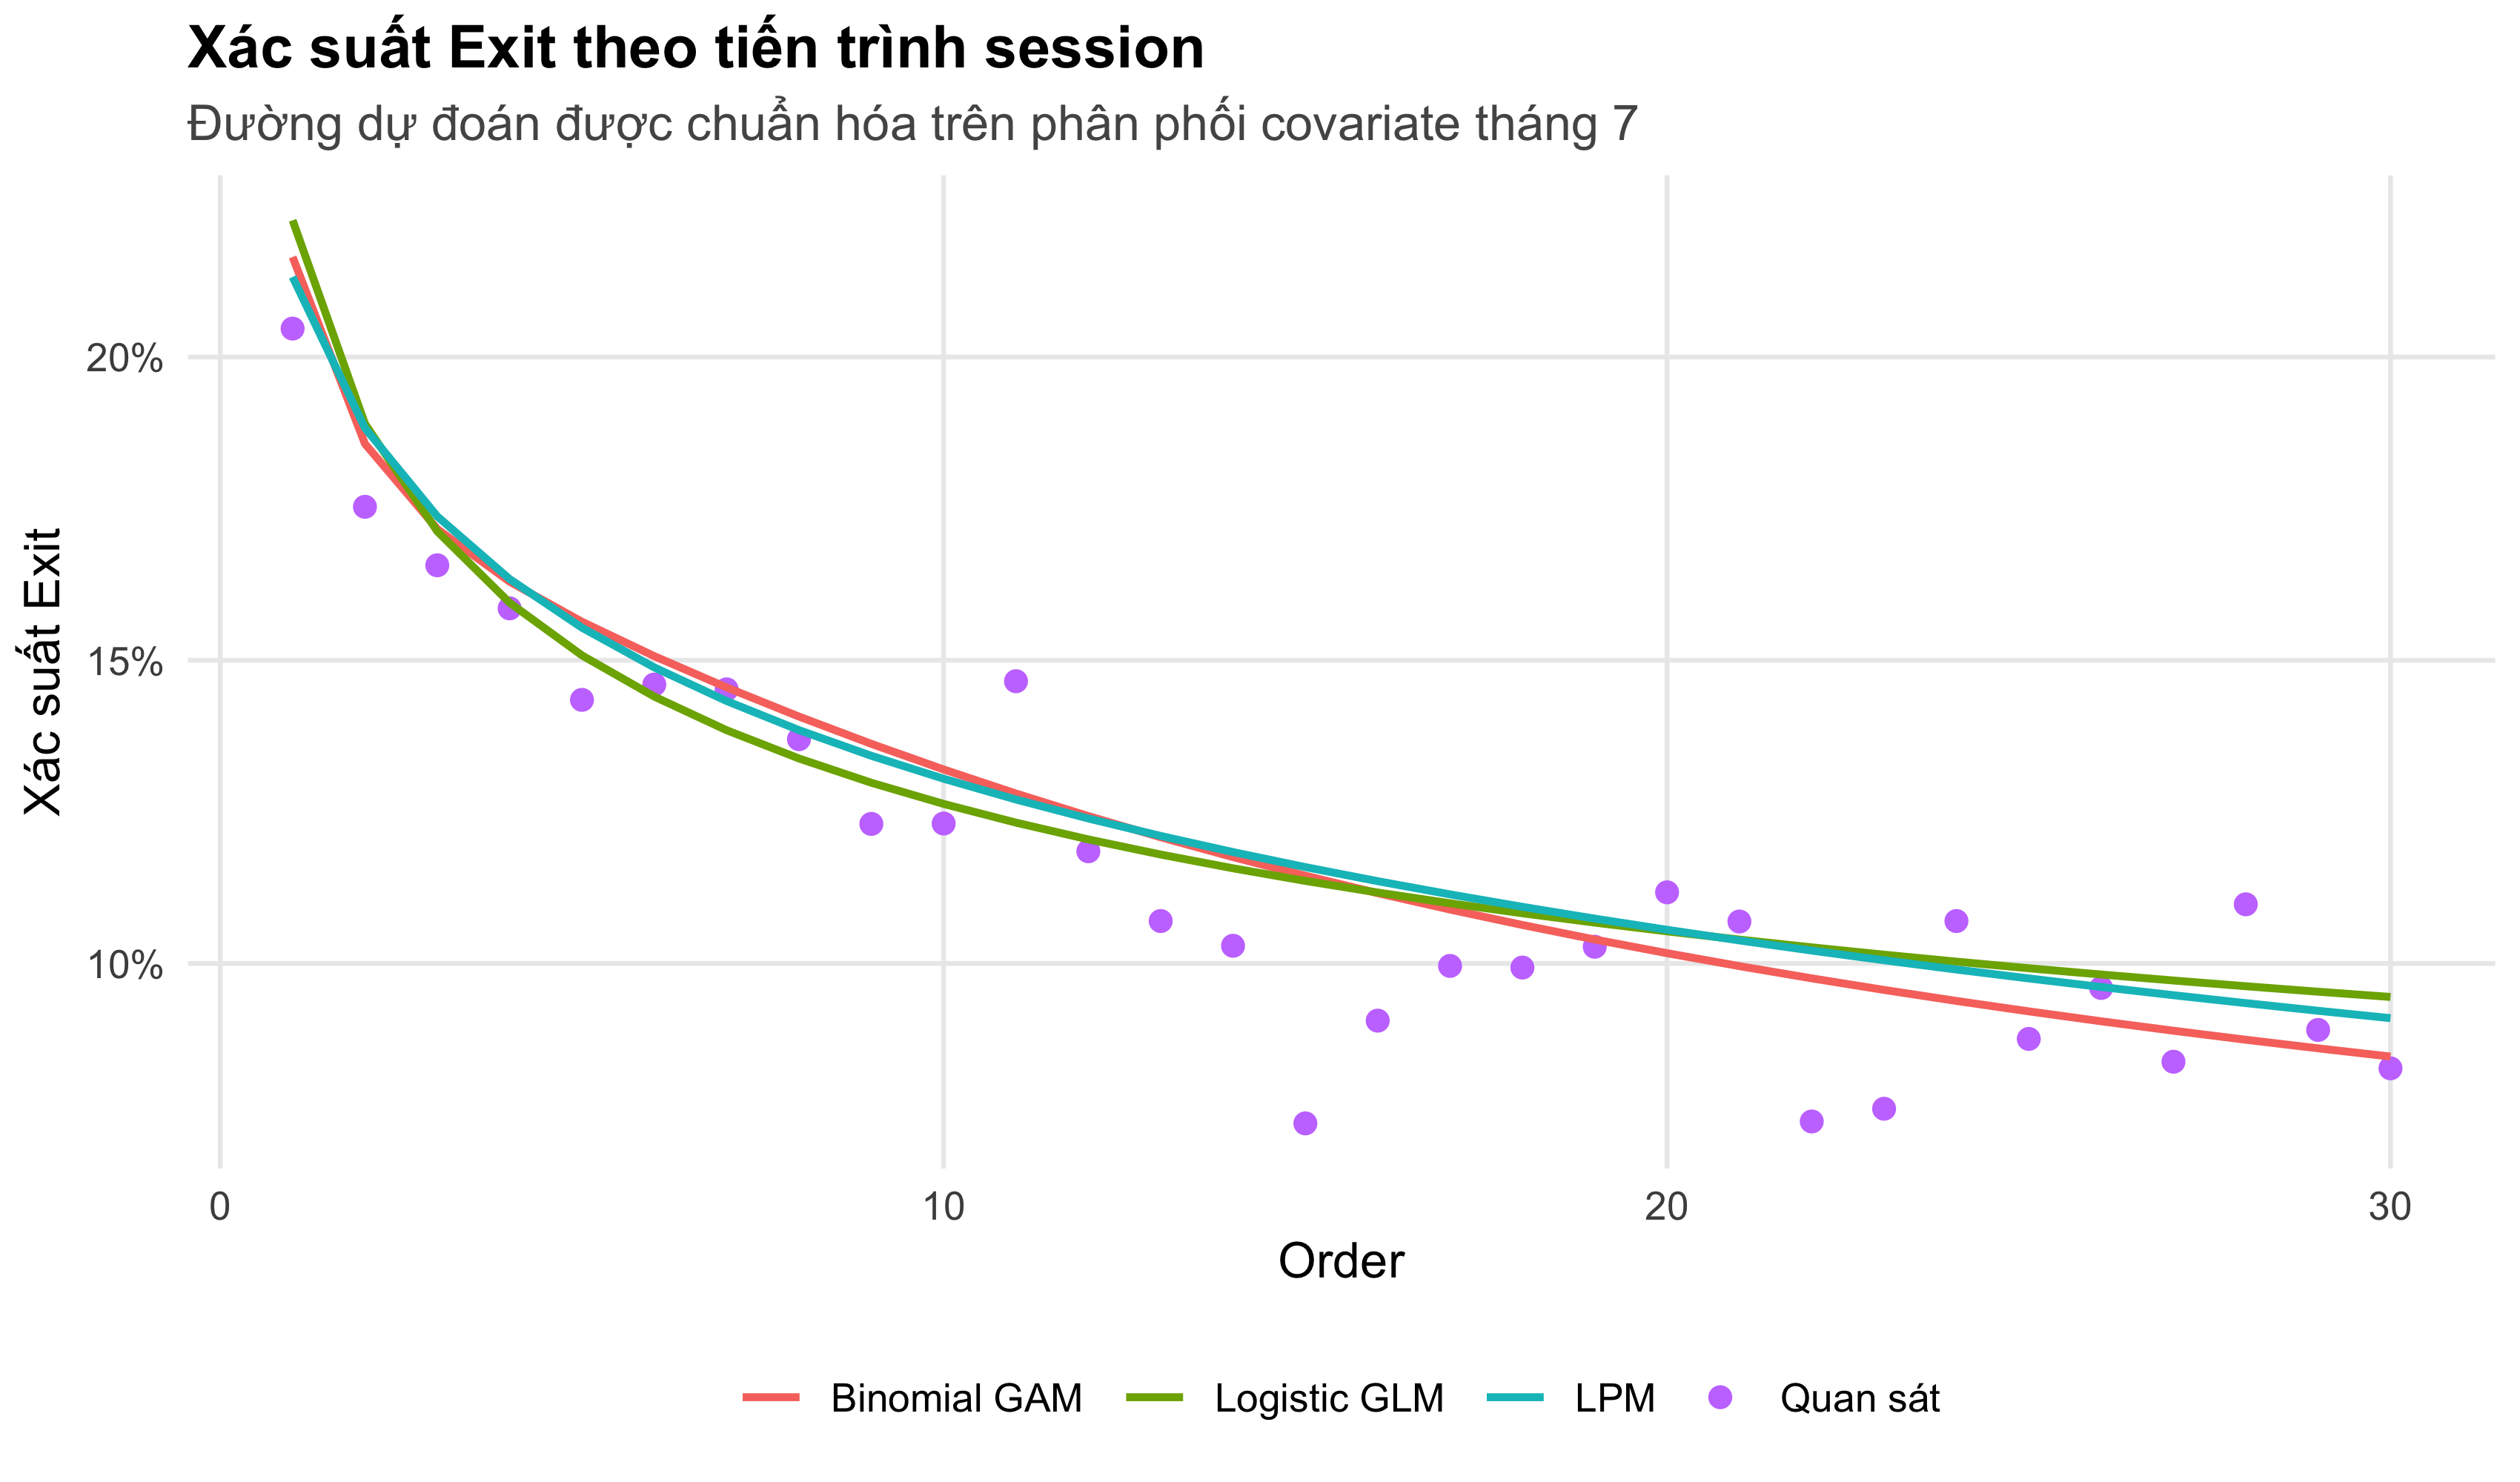
\includegraphics[width=\textwidth]{img/fig-order-probability.png}
\caption{Xác suất Exit quan sát và dự đoán theo tiến trình session; ba đường dự
đoán được chuẩn hóa trên phân phối covariate tháng 7}
\label{fig:order-probability}
\end{figure}

Hình~\ref{fig:order-probability} là căn cứ để trả lời câu hỏi liệu quan hệ tuyến
tính có đủ hay cần đến GAM. Ba đường dự đoán gần như trùng nhau trong khoảng
\texttt{order} từ 1 đến 20; chỉ ở phần đuôi đường GAM mới tách xuống thấp hơn hai
dạng tuyến tính. Nói cách khác, sau phép biến đổi $\log_2$, dạng hàm tuyến tính
đã nắm bắt gần trọn quan hệ và phần phi tuyến còn lại là nhỏ. Các điểm quan sát ở
đuôi dao động mạnh hơn đơn giản vì số session còn tồn tại giảm dần.

\subsection{Kết quả mô hình dự đoán: giá trị bổ sung của các nhóm biến}

Bảng~\ref{tab:model-compare} so sánh chín mô hình (ba phương pháp $\times$ ba
tầng predictor) trên cùng tập validation tháng 7.

\begin{table}[H]
\centering
\caption{So sánh ba tầng predictor của ba phương pháp trên validation tháng 7}
\label{tab:model-compare}
\footnotesize
\setlength{\tabcolsep}{4pt}
\begin{tabular}{llrrrrrrrl}
\toprule
\textbf{Phương pháp} & \textbf{Tầng predictor} & \textbf{ROC--AUC}
& \textbf{AP} & \textbf{Log loss} & \textbf{Brier} & \textbf{Brier skill}
& \textbf{Cal. int.} & \textbf{Cal. slope} & \textbf{AIC} \\
\midrule
LPM      & Baseline         & 0,589 & 0,179 & 0,406 & 0,122 & 0,010 & $-$0,066 & 0,899 & Không so sánh \\
LPM      & Current-click    & 0,611 & 0,197 & 0,405 & 0,121 & 0,016 & $-$0,067 & 0,808 & Không so sánh \\
LPM      & History-enhanced & 0,660 & 0,233 & 0,397 & 0,119 & 0,038 & $-$0,060 & 0,755 & Không so sánh \\
\midrule
Logistic & Baseline         & 0,589 & 0,179 & 0,407 & 0,122 & 0,010 & $-$0,065 & 0,880 & 94.998,4 \\
Logistic & Current-click    & 0,611 & 0,199 & 0,403 & 0,121 & 0,016 & $-$0,068 & 0,873 & 94.222,0 \\
Logistic & History-enhanced & 0,662 & 0,237 & 0,392 & 0,118 & 0,039 & $-$0,059 & 0,922 & 91.801,3 \\
\midrule
GAM      & Baseline         & 0,589 & 0,179 & 0,406 & 0,122 & 0,010 & $-$0,064 & 0,879 & 94.957,6 \\
GAM      & Current-click    & 0,612 & 0,199 & 0,403 & 0,121 & 0,016 & $-$0,067 & 0,864 & 94.160,7 \\
GAM      & History-enhanced & 0,662 & 0,238 & 0,392 & 0,118 & 0,040 & $-$0,057 & 0,932 & 91.746,6 \\
\bottomrule
\end{tabular}

\vspace{4pt}
{\footnotesize AP = Average Precision; Cal. int. = calibration intercept;
Cal. slope = calibration slope. AIC của LPM để trống vì mô hình Gaussian không
cùng họ likelihood với hai mô hình nhị phân nên không so sánh được.}
\end{table}

Cả hai bước bổ sung biến đều có ý nghĩa thống kê. Kiểm định Wald robust chung cho
nhóm \texttt{Price + Category + Colour + Location + Photography + Page} cho
$p < 0{,}001$ trong cả LPM và Logistic GLM. Sau khi đã có các biến current-click,
nhóm biến lịch sử tiếp tục bổ sung với robust joint $p < 0{,}001$.

Điều đáng chú ý là \emph{độ lớn} của hai bước rất khác nhau. Thêm toàn bộ đặc
điểm sản phẩm chỉ nâng ROC--AUC của Logistic GLM từ 0,589 lên 0,611 và giảm log
loss 0,004. Trong khi đó nhóm biến lịch sử duyệt nâng ROC--AUC tiếp lên 0,662 và
giảm log loss thêm 0,012 -- gấp ba lần đóng góp của đặc điểm sản phẩm.\footnote{%
Các mức tăng/giảm được tính trên giá trị chưa làm tròn ($+0{,}050$ ROC--AUC và
$-0{,}012$ log loss), nên có thể lệch một đơn vị ở chữ số thập phân thứ ba so với
hiệu của hai giá trị đã làm tròn trong Bảng~\ref{tab:model-compare}.}
Kết luận thực nghiệm: \textbf{hành vi đã diễn ra trong session mang nhiều thông
tin dự báo hơn hẳn đặc điểm của riêng click hiện tại}.

\begin{table}[H]
\centering
\caption{Mười hai nhóm biến có bằng chứng liên hệ mạnh nhất trong Logistic GLM
history-enhanced (Wald robust theo cụm session)}
\label{tab:terms}
\small
\begin{tabular}{lrrll}
\toprule
\textbf{Nhóm biến} & \textbf{Wald $\chi^2$} & \textbf{df} & \textbf{p-value}
& \textbf{Hiệu ứng / CI 95\%} \\
\midrule
$\log_2(\text{Order})$              & 1081,19 & 1  & $< 0{,}001$ & OR 0,640 (0,623--0,657) \\
Số danh mục duy nhất đến hiện tại   & 639,64  & 1  & $< 0{,}001$ & OR 1,562 (1,509--1,617) \\
Quay lại sản phẩm cũ                & 469,92  & 1  & $< 0{,}001$ & OR 2,218 (2,064--2,384) \\
Page                                & 465,93  & 4  & $< 0{,}001$ & Joint test \\
Country                             & 150,60  & 17 & $< 0{,}001$ & Joint test \\
Colour                              & 93,18   & 13 & $< 0{,}001$ & Joint test \\
Chuyển Category ở click hiện tại    & 75,32   & 1  & $< 0{,}001$ & OR 1,311 (1,233--1,394) \\
Category                            & 48,63   & 3  & $< 0{,}001$ & Joint test \\
Chuyển Page ở click hiện tại        & 46,80   & 1  & $< 0{,}001$ & OR 1,169 (1,118--1,223) \\
Số sản phẩm duy nhất đến hiện tại   & 40,78   & 1  & $< 0{,}001$ & OR 0,988 (0,984--0,991) \\
Location                            & 32,76   & 5  & $< 0{,}001$ & Joint test \\
Price (mỗi 10 USD)                  & 6,96    & 1  & 0,008       & OR 1,032 (1,008--1,056) \\
\bottomrule
\end{tabular}
\end{table}

Năm nhóm biến đứng đầu theo p-value robust và thống kê Wald trên mỗi bậc tự do
là: $\log_2(\text{Order})$, số danh mục duy nhất đã xem, hành vi quay lại sản
phẩm cũ, \texttt{Page} và \texttt{Country}. Ba hiệu ứng đơn biến đáng chú ý:

\begin{itemize}
  \item Mỗi lần \texttt{order} tăng gấp đôi, odds kết thúc session nhân với
  0,640 -- session càng đi sâu càng ít có khả năng dừng ở click kế tiếp.
  \item Click vào một sản phẩm \emph{đã xem trước đó} trong cùng session có odds
  kết thúc cao gấp 2,218 lần, hiệu ứng đơn biến lớn nhất trong mô hình.
  \item Mỗi danh mục mới được xem thêm làm odds kết thúc nhân với 1,562.
\end{itemize}

Ngược lại, \texttt{Price} tuy có ý nghĩa thống kê ($p = 0{,}008$) nhưng hiệu ứng
rất nhỏ: OR 1,032 cho mỗi 10 USD. Cần nhấn mạnh rằng thứ hạng trong
Bảng~\ref{tab:terms} phản ánh \emph{bằng chứng về liên hệ}, không phải mức độ
quan trọng nhân quả, và không nên so sánh trực tiếp độ lớn OR giữa các biến có
đơn vị khác nhau.

\begin{figure}[H]
\centering
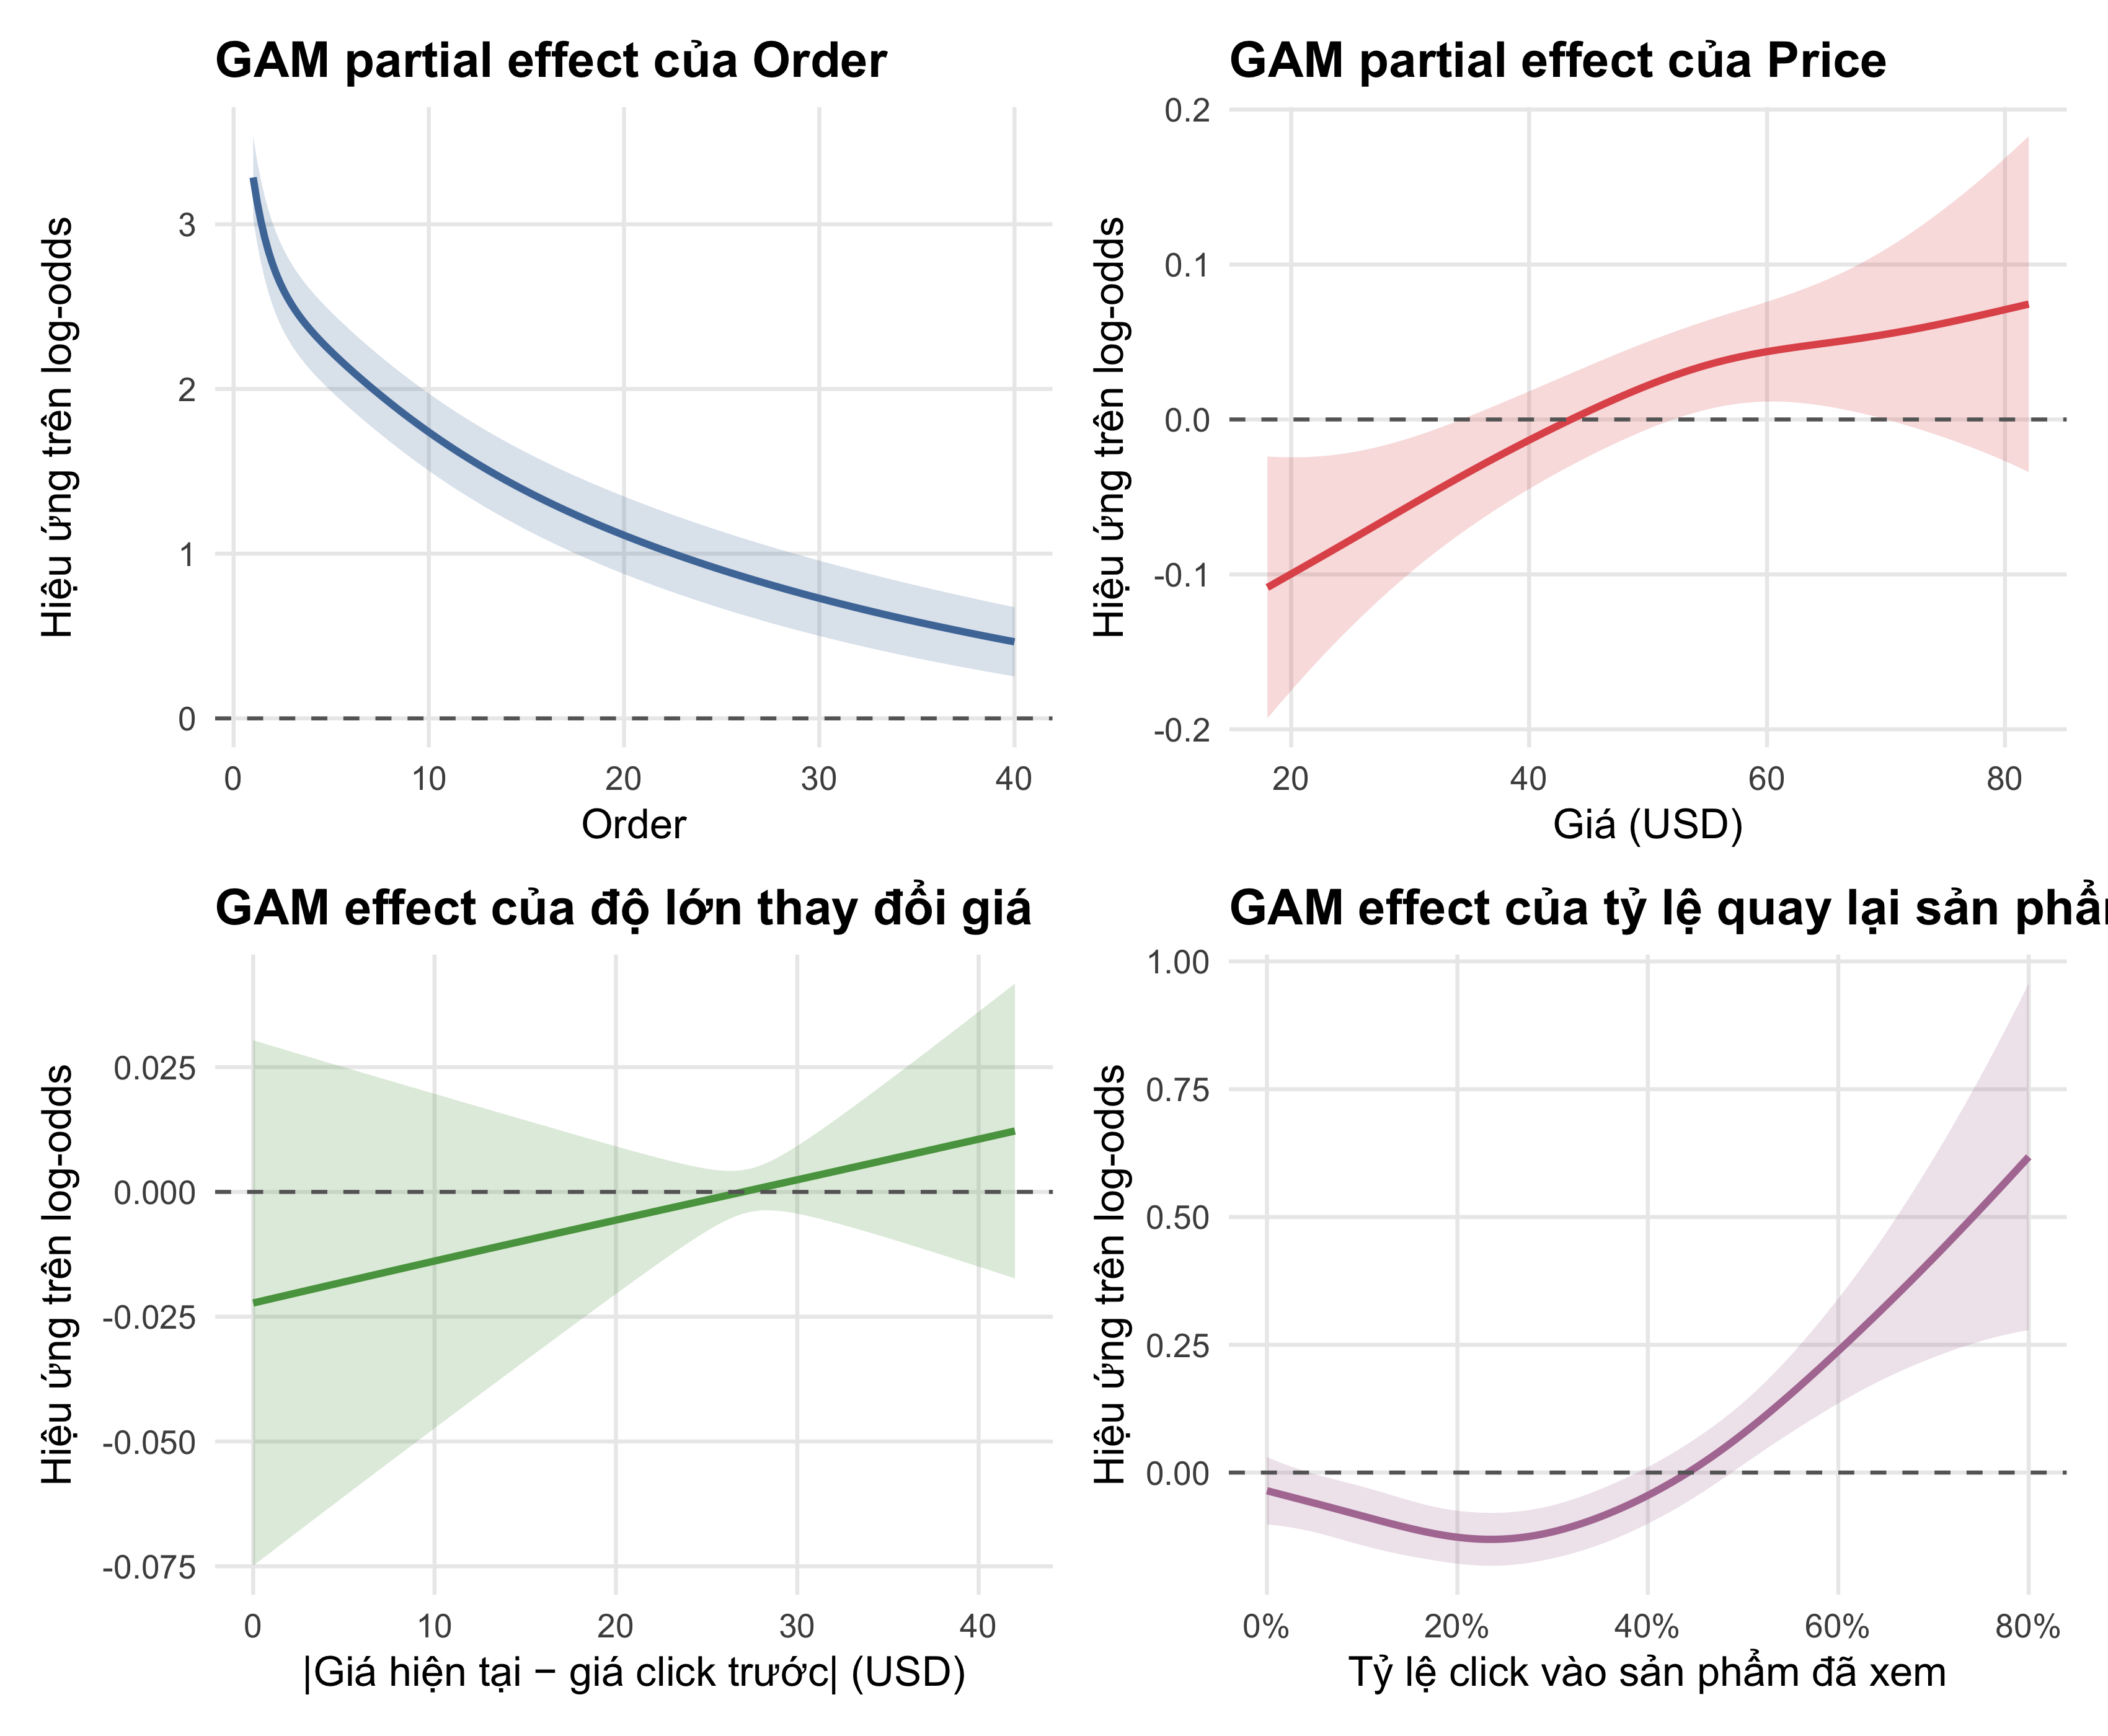
\includegraphics[width=\textwidth]{img/fig-gam-smooths.png}
\caption{Các hàm trơn của GAM history-enhanced: partial effect của Order, Price,
độ lớn thay đổi giá và tỷ lệ quay lại sản phẩm (thang log-odds)}
\label{fig:gam-smooths}
\end{figure}

Hình~\ref{fig:gam-smooths} minh họa dạng hàm mà GAM ước lượng. Hàm trơn của
\texttt{Order} giảm đơn điệu và gần tuyến tính trên thang $\log_2$, phù hợp với
Hình~\ref{fig:order-probability}. Tuy nhiên, như phần chẩn đoán dưới đây chỉ ra,
các partial-effect plot này \textbf{không} được diễn giải như hiệu ứng riêng biệt
của từng biến vì mức concurvity giữa các term rất cao.

\subsection{Chẩn đoán mô hình}

\begin{table}[H]
\centering
\caption{Kiểm tra kích thước basis của GAM history-enhanced}
\label{tab:kcheck}
\small
\begin{tabular}{lrrrr}
\toprule
\textbf{Hàm trơn} & \textbf{$k'$} & \textbf{edf} & \textbf{k-index} & \textbf{p-value} \\
\midrule
s(log2\_order)         & 9,0 & 4,52 & 0,934 & 0,170 \\
s(price)               & 7,0 & 1,88 & 0,943 & 0,350 \\
s(repeat\_rate)        & 7,0 & 3,20 & 0,950 & 0,580 \\
s(abs\_price\_delta\_10) & 7,0 & 1,01 & 0,947 & 0,362 \\
\bottomrule
\end{tabular}
\end{table}

Không hàm trơn nào có edf tiến sát giới hạn basis $k'$ và mọi p-value đều lớn hơn
0,05, nên kích thước basis đã đủ. Đáng chú ý là
$\text{edf} = 1{,}01$ cho \texttt{s(abs\_price\_delta\_10)} và $1{,}88$ cho
\texttt{s(price)} -- hai hàm này gần như tuyến tính, tức GAM hầu như không tìm
thấy phi tuyến đáng kể ở các biến giá.

\begin{table}[H]
\centering
\caption{Mười GVIF điều chỉnh lớn nhất của Logistic GLM (trái) và năm cặp term
có concurvity cao nhất trong GAM (phải)}
\label{tab:collinearity}
\small
\begin{minipage}[t]{0.46\textwidth}
\centering
\begin{tabular}{lr}
\toprule
\textbf{Term} & \textbf{GVIF điều chỉnh} \\
\midrule
log2\_order             & 2,424 \\
unique\_products        & 2,022 \\
price\_vs\_prior\_mean\_10 & 1,989 \\
unique\_categories      & 1,944 \\
price\_10               & 1,729 \\
price\_delta\_10        & 1,688 \\
category\_switch\_rate  & 1,627 \\
repeat\_rate            & 1,497 \\
category\_switch        & 1,442 \\
repeat\_current         & 1,441 \\
\bottomrule
\end{tabular}
\end{minipage}
\hfill
\begin{minipage}[t]{0.50\textwidth}
\centering
\begin{tabular}{llr}
\toprule
\textbf{Term} & \textbf{Term còn lại} & \textbf{Concurvity} \\
\midrule
s(log2\_order)          & para           & 0,994 \\
s(abs\_price\_delta\_10) & para           & 0,966 \\
s(repeat\_rate)         & para           & 0,866 \\
s(log2\_order)          & s(repeat\_rate) & 0,802 \\
para                    & s(repeat\_rate) & 0,769 \\
\bottomrule
\end{tabular}
\end{minipage}
\end{table}

Hai chẩn đoán này cho hai kết luận trái ngược nhau và cần được đọc riêng.
Với Logistic GLM, GVIF điều chỉnh lớn nhất chỉ 2,424, thấp hơn nhiều ngưỡng cảnh
báo thông thường, nên đa cộng tuyến không phải vấn đề với các hệ số trong
Bảng~\ref{tab:terms}. Ngược lại, concurvity trong GAM lên tới 0,994 -- gần mức
xác định hoàn toàn. Nhóm đã loại \texttt{s(unique\_products)} khỏi GAM vì gần
trùng thông tin với \texttt{Order} và \texttt{repeat\_rate}, nhưng concurvity còn
lại vẫn quá cao. Vì vậy GAM chỉ được giữ làm \emph{đối chứng dự báo phi tuyến},
còn các partial-effect plot của nó không được dùng làm bằng chứng về hiệu ứng
riêng của từng biến.

\begin{figure}[H]
\centering
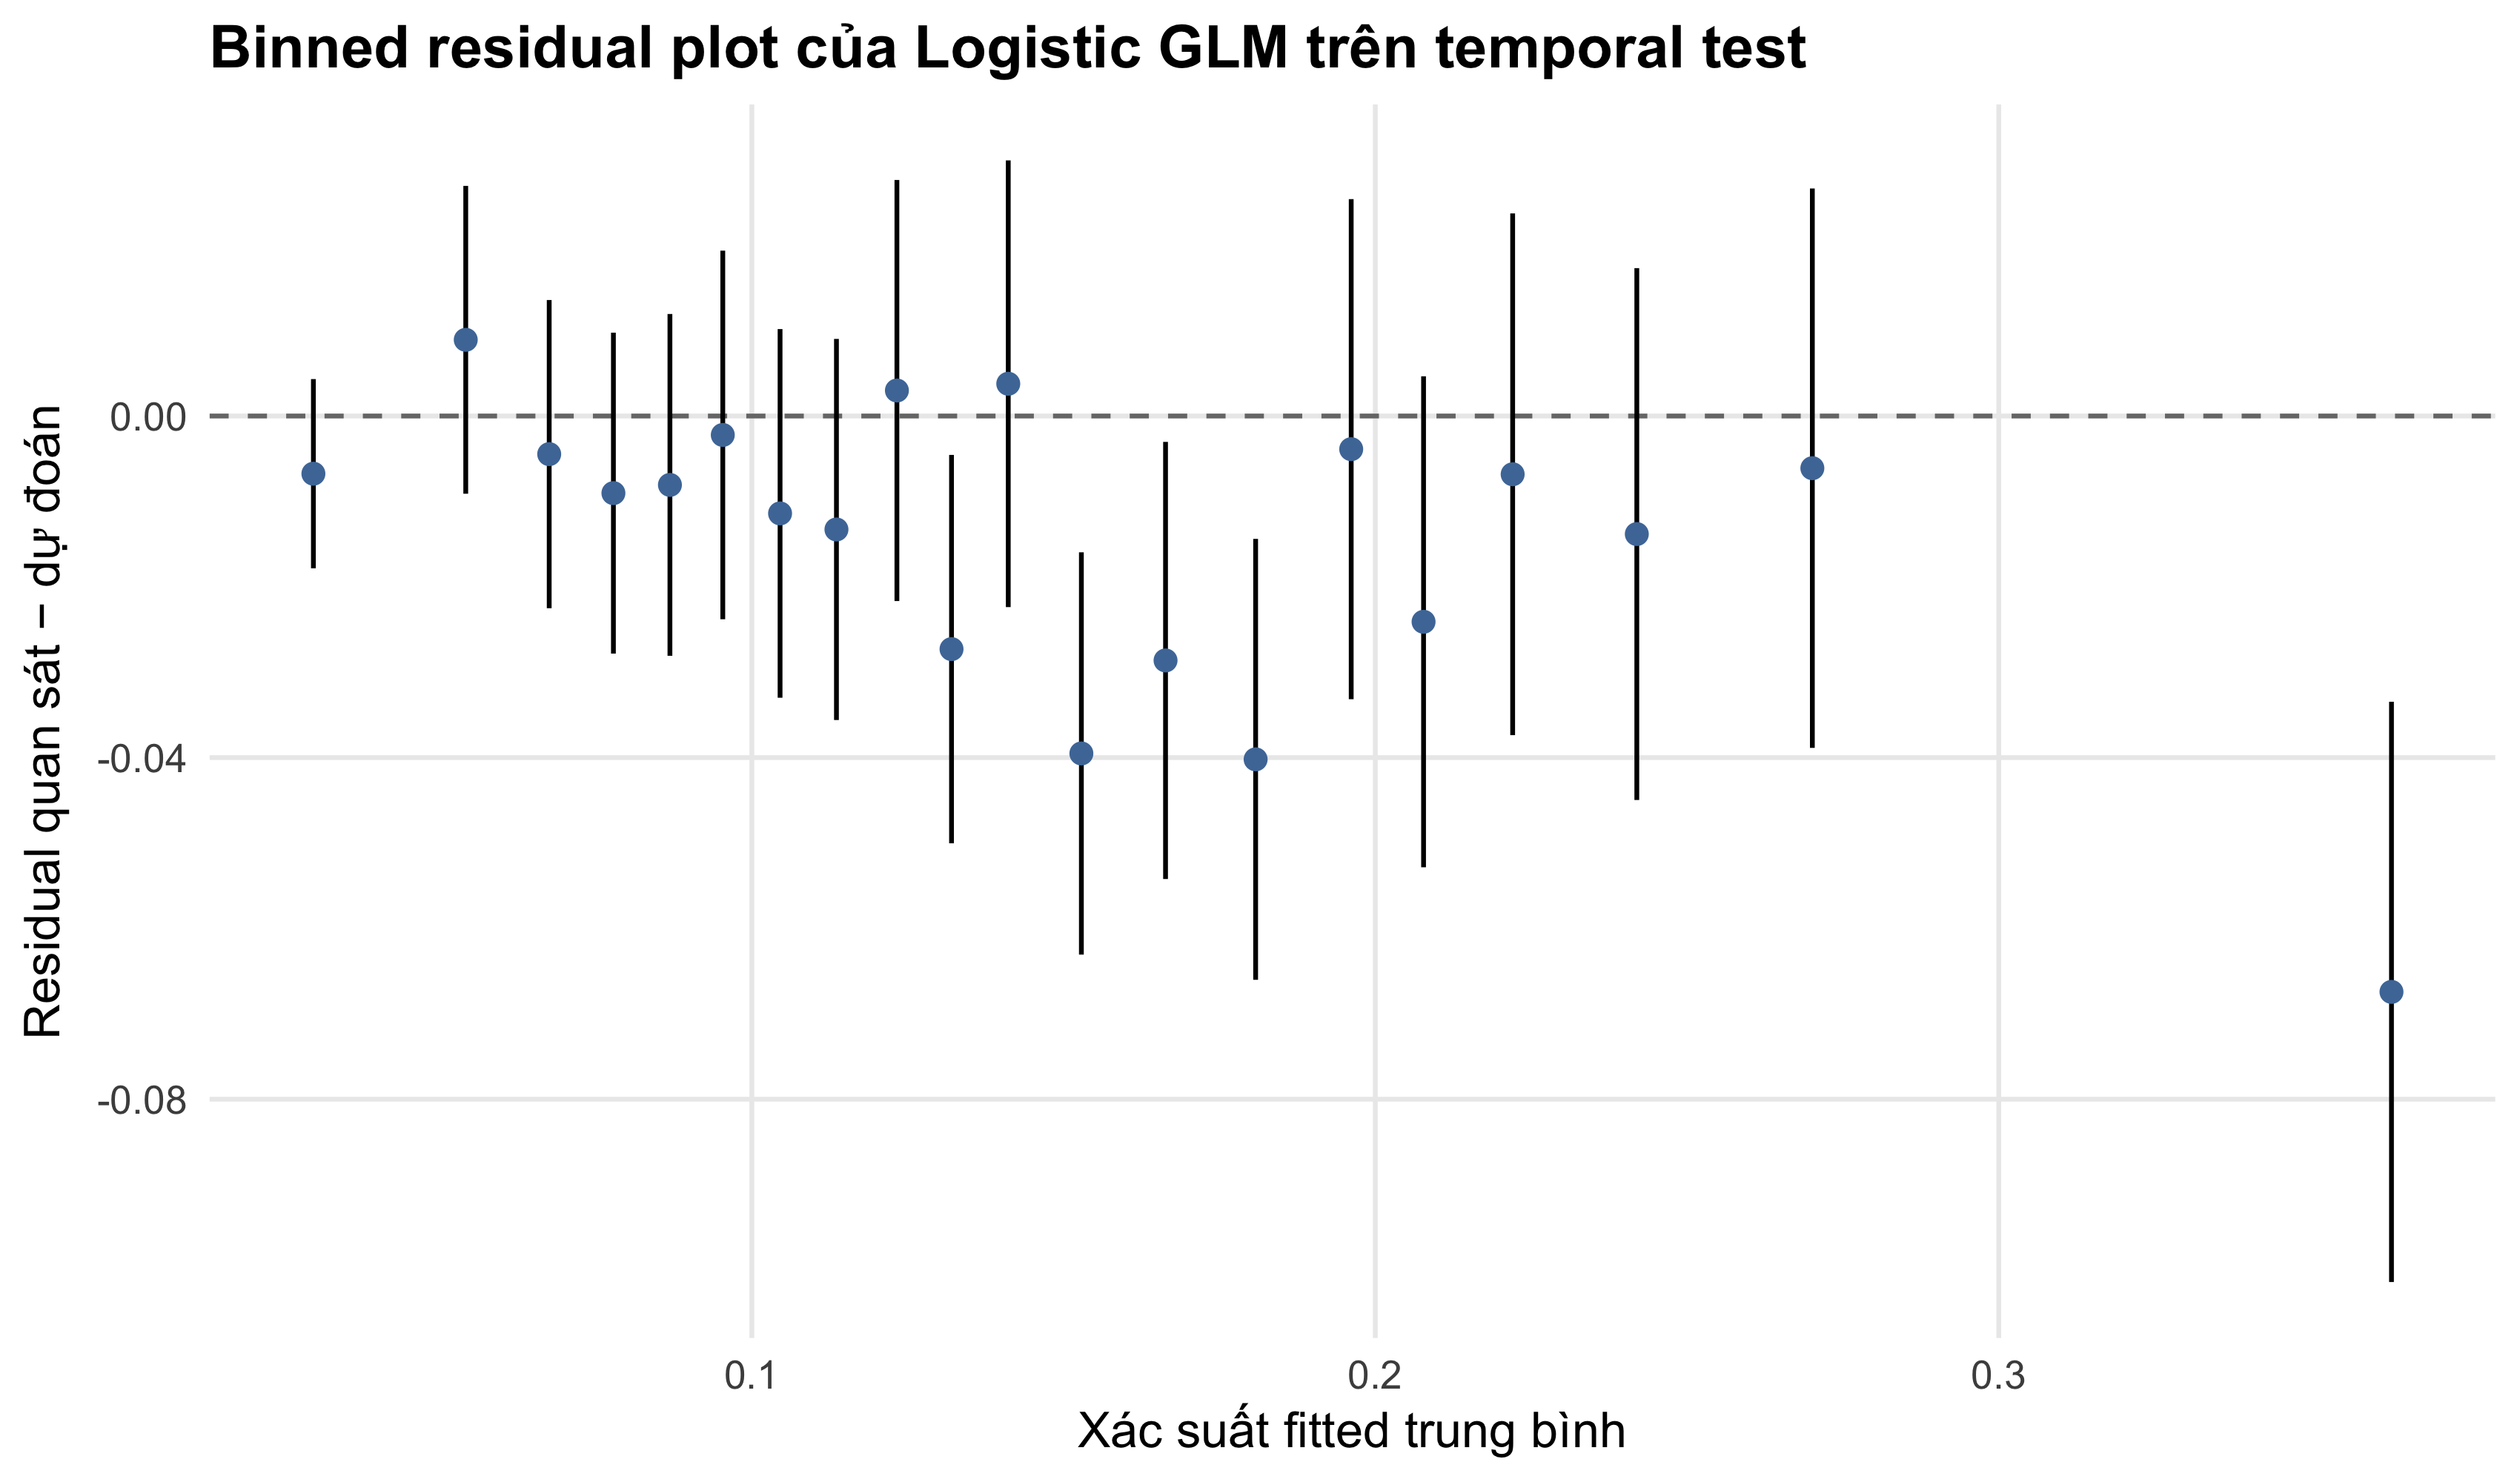
\includegraphics[width=0.85\textwidth]{img/fig-binned-residual.png}
\caption{Binned residual plot của Logistic GLM trên temporal test 01--12/08}
\label{fig:binned-residual}
\end{figure}

Với outcome nhị phân, đồ thị phần dư thông thường của hồi quy tuyến tính không có
ý nghĩa, nên nhóm dùng binned residual plot~\cite{gelman2007}: dữ liệu được chia
thành 20 nhóm theo
xác suất dự đoán và vẽ residual trung bình của mỗi nhóm kèm sai số chuẩn. Phần
lớn các điểm nằm quanh đường 0 với khoảng sai số phủ 0, nghĩa là không có sai
lệch hệ thống rõ rệt theo mức xác suất dự đoán.

\subsection{Kết quả mô hình phân loại: so sánh ba phương pháp}

\subsubsection{Các metric được sử dụng}

Với quan sát $i = 1,\ldots,n$, ký hiệu $y_i \in \{0,1\}$ là nhãn \texttt{Exit}
thực tế và $\hat p_i = P(Y_i = 1 \mid X_i)$ là xác suất do mô hình dự đoán. Báo
cáo đánh giá hai khía cạnh tách biệt: \emph{chất lượng xác suất} và \emph{chất
lượng phân loại sau khi chọn threshold}.

\textbf{Nhóm metric không phụ thuộc threshold.}

\begin{itemize}
  \item \textbf{ROC--AUC} là diện tích dưới đường ROC. Tương đương,
  \[
  \operatorname{AUC} = P(\hat p_{+} > \hat p_{-}) + \tfrac{1}{2}P(\hat p_{+} = \hat p_{-}),
  \]
  với $\hat p_{+}$, $\hat p_{-}$ là xác suất dự đoán của một quan sát dương và
  một quan sát âm lấy ngẫu nhiên. AUC bằng 0,5 tương ứng xếp hạng ngẫu nhiên;
  càng gần 1 càng tốt. Metric này chỉ đo khả năng \emph{xếp hạng}.

  \item \textbf{Average Precision (AP)} tóm tắt đường Precision--Recall,
  $\operatorname{AP} = \sum_k (R_k - R_{k-1}) P_k$. Mốc tham chiếu của mô hình
  ngẫu nhiên xấp xỉ bằng prevalence của \texttt{Exit}. AP được báo cáo cùng AUC
  vì ROC có thể quá lạc quan khi lớp dương chiếm thiểu số.

  \item \textbf{Log loss} đánh giá trực tiếp xác suất dự đoán:
  \[
  -\frac{1}{n}\sum_{i=1}^{n}\left[y_i\log(\hat p_i) + (1-y_i)\log(1-\hat p_i)\right].
  \]
  Càng nhỏ càng tốt; phạt rất nặng các dự đoán tự tin nhưng sai.

  \item \textbf{Brier score} là sai số bình phương trung bình của xác suất,
  $\operatorname{Brier} = \frac{1}{n}\sum_{i=1}^{n}(\hat p_i - y_i)^2$.
  \textbf{Brier Skill Score} so sánh với dự báo hằng bằng prevalence train:
  $\operatorname{BSS} = 1 - \operatorname{Brier}_{model}/\operatorname{Brier}_{ref}$.
  BSS $> 0$ nghĩa là tốt hơn mô hình tham chiếu.

  \item \textbf{Calibration intercept và slope} được ước lượng từ
  $\operatorname{logit}\{P(Y=1)\} = \alpha + \beta\operatorname{logit}(\hat p)$.
  Mô hình hiệu chỉnh lý tưởng có $\alpha = 0$ và $\beta = 1$. Intercept âm cho
  thấy mô hình dự đoán xác suất thiên cao; slope nhỏ hơn 1 cho thấy dự đoán quá
  cực đoan.
\end{itemize}

\textbf{Nhóm metric phụ thuộc threshold.} Sau khi chọn threshold $t$, dự đoán
dương khi $\hat p_i \geq t$. Với $TP, TN, FP, FN$ là số dương đúng, âm đúng,
dương giả và âm giả:

\[
\begin{aligned}
\operatorname{Accuracy} &= \frac{TP+TN}{TP+TN+FP+FN}, &
\operatorname{Precision} &= \frac{TP}{TP+FP}, \\
\operatorname{Recall\ (Sensitivity)} &= \frac{TP}{TP+FN}, &
\operatorname{Specificity} &= \frac{TN}{TN+FP}, \\
F_1 &= 2\,\frac{\operatorname{Precision}\times\operatorname{Recall}}
{\operatorname{Precision}+\operatorname{Recall}}. & &
\end{aligned}
\]

\subsubsection{Lựa chọn mô hình trên validation}

\begin{table}[H]
\centering
\caption{Metric validation tháng 7 dùng để lựa chọn mô hình}
\label{tab:validation}
\small
\begin{tabular}{lrrrrrrr}
\toprule
\textbf{Model} & \textbf{ROC--AUC} & \textbf{AP} & \textbf{Log loss}
& \textbf{Brier} & \textbf{Brier skill} & \textbf{Cal. int.} & \textbf{Cal. slope} \\
\midrule
LPM          & 0,660 & 0,233 & 0,397 & 0,119 & 0,038 & $-$0,060 & 0,755 \\
Logistic GLM & 0,662 & 0,237 & 0,392 & 0,118 & 0,039 & $-$0,059 & 0,922 \\
Binomial GAM & 0,662 & 0,238 & 0,392 & 0,118 & 0,040 & $-$0,057 & 0,932 \\
\bottomrule
\end{tabular}
\end{table}

Quy tắc lựa chọn được xác định \emph{trước} khi nhìn kết quả: giữ lại các mô hình
nằm trong 1\% log loss tốt nhất, rồi trong 1\% Brier tốt nhất; nếu vẫn còn nhiều
ứng viên thì ưu tiên Logistic GLM vì đơn giản và dễ diễn giải hơn GAM, còn LPM
chỉ đóng vai trò benchmark. Logistic GLM và Binomial GAM có log loss và Brier
giống nhau đến ba chữ số thập phân, nên cả hai cùng vào nhóm gần tương đương và
\textbf{Logistic GLM được chọn}. Threshold tối đa $F_1$ của từng mô hình được
chốt từ prediction out-of-fold của five-fold CV theo session trên tập train,
trước khi mở temporal test.

\subsubsection{Hiệu năng cuối trên temporal test}

\begin{table}[H]
\centering
\caption{Hiệu năng cuối của ba mô hình trên temporal test 01--12/08; khoảng tin
cậy 95\% từ 500 lần cluster bootstrap theo session}
\label{tab:final-metrics}
\footnotesize
\setlength{\tabcolsep}{4pt}
\begin{tabular}{llllrlrrr}
\toprule
\textbf{Model} & \textbf{ROC--AUC} & \textbf{AP} & \textbf{Log loss}
& \textbf{BSS} & \textbf{Brier} & \textbf{Cal. int.} & \textbf{Cal. slope}
& \textbf{Ngoài $[0,1]$} \\
\midrule
LPM          & 0,662 (0,644--0,681) & 0,224 (0,212--0,241) & 0,382 (0,363--0,399) & 0,036 & 0,114 (0,107--0,120) & $-$0,138 & 0,868 & 1,706\% \\
Logistic GLM & 0,666 (0,647--0,685) & 0,230 (0,218--0,246) & 0,379 (0,361--0,396) & 0,039 & 0,113 (0,107--0,119) & $-$0,127 & 0,934 & 0,000\% \\
Binomial GAM & 0,666 (0,647--0,686) & 0,230 (0,218--0,247) & 0,379 (0,361--0,396) & 0,039 & 0,113 (0,107--0,119) & $-$0,125 & 0,942 & 0,000\% \\
\bottomrule
\end{tabular}
\end{table}

Ba mô hình gần như không phân biệt được về khả năng xếp hạng: khoảng tin cậy
ROC--AUC chồng lấn gần hoàn toàn. Khác biệt thực chất nằm ở hai chỗ khác. Thứ
nhất, \textbf{calibration slope}: LPM chỉ đạt 0,868 trong khi Logistic GLM đạt
0,934 và GAM đạt 0,942 -- xác suất của LPM cực đoan hơn mức dữ liệu cho phép.
Thứ hai, \textbf{tính hợp lệ của xác suất}: LPM sinh ra 1,706\% dự đoán nằm ngoài
khoảng $[0,1]$, tức những giá trị không thể diễn giải như xác suất; hai mô hình
nhị phân theo cấu trúc không bao giờ mắc lỗi này.

Brier Skill Score của cả ba mô hình chỉ nằm trong khoảng 0,036--0,039, nghĩa là
chúng chỉ tốt hơn dự báo hằng bằng prevalence khoảng 4\%. Đây là mức cải thiện
khiêm tốn và cần được nêu rõ thay vì che đi sau con số AUC.

\begin{figure}[H]
\centering
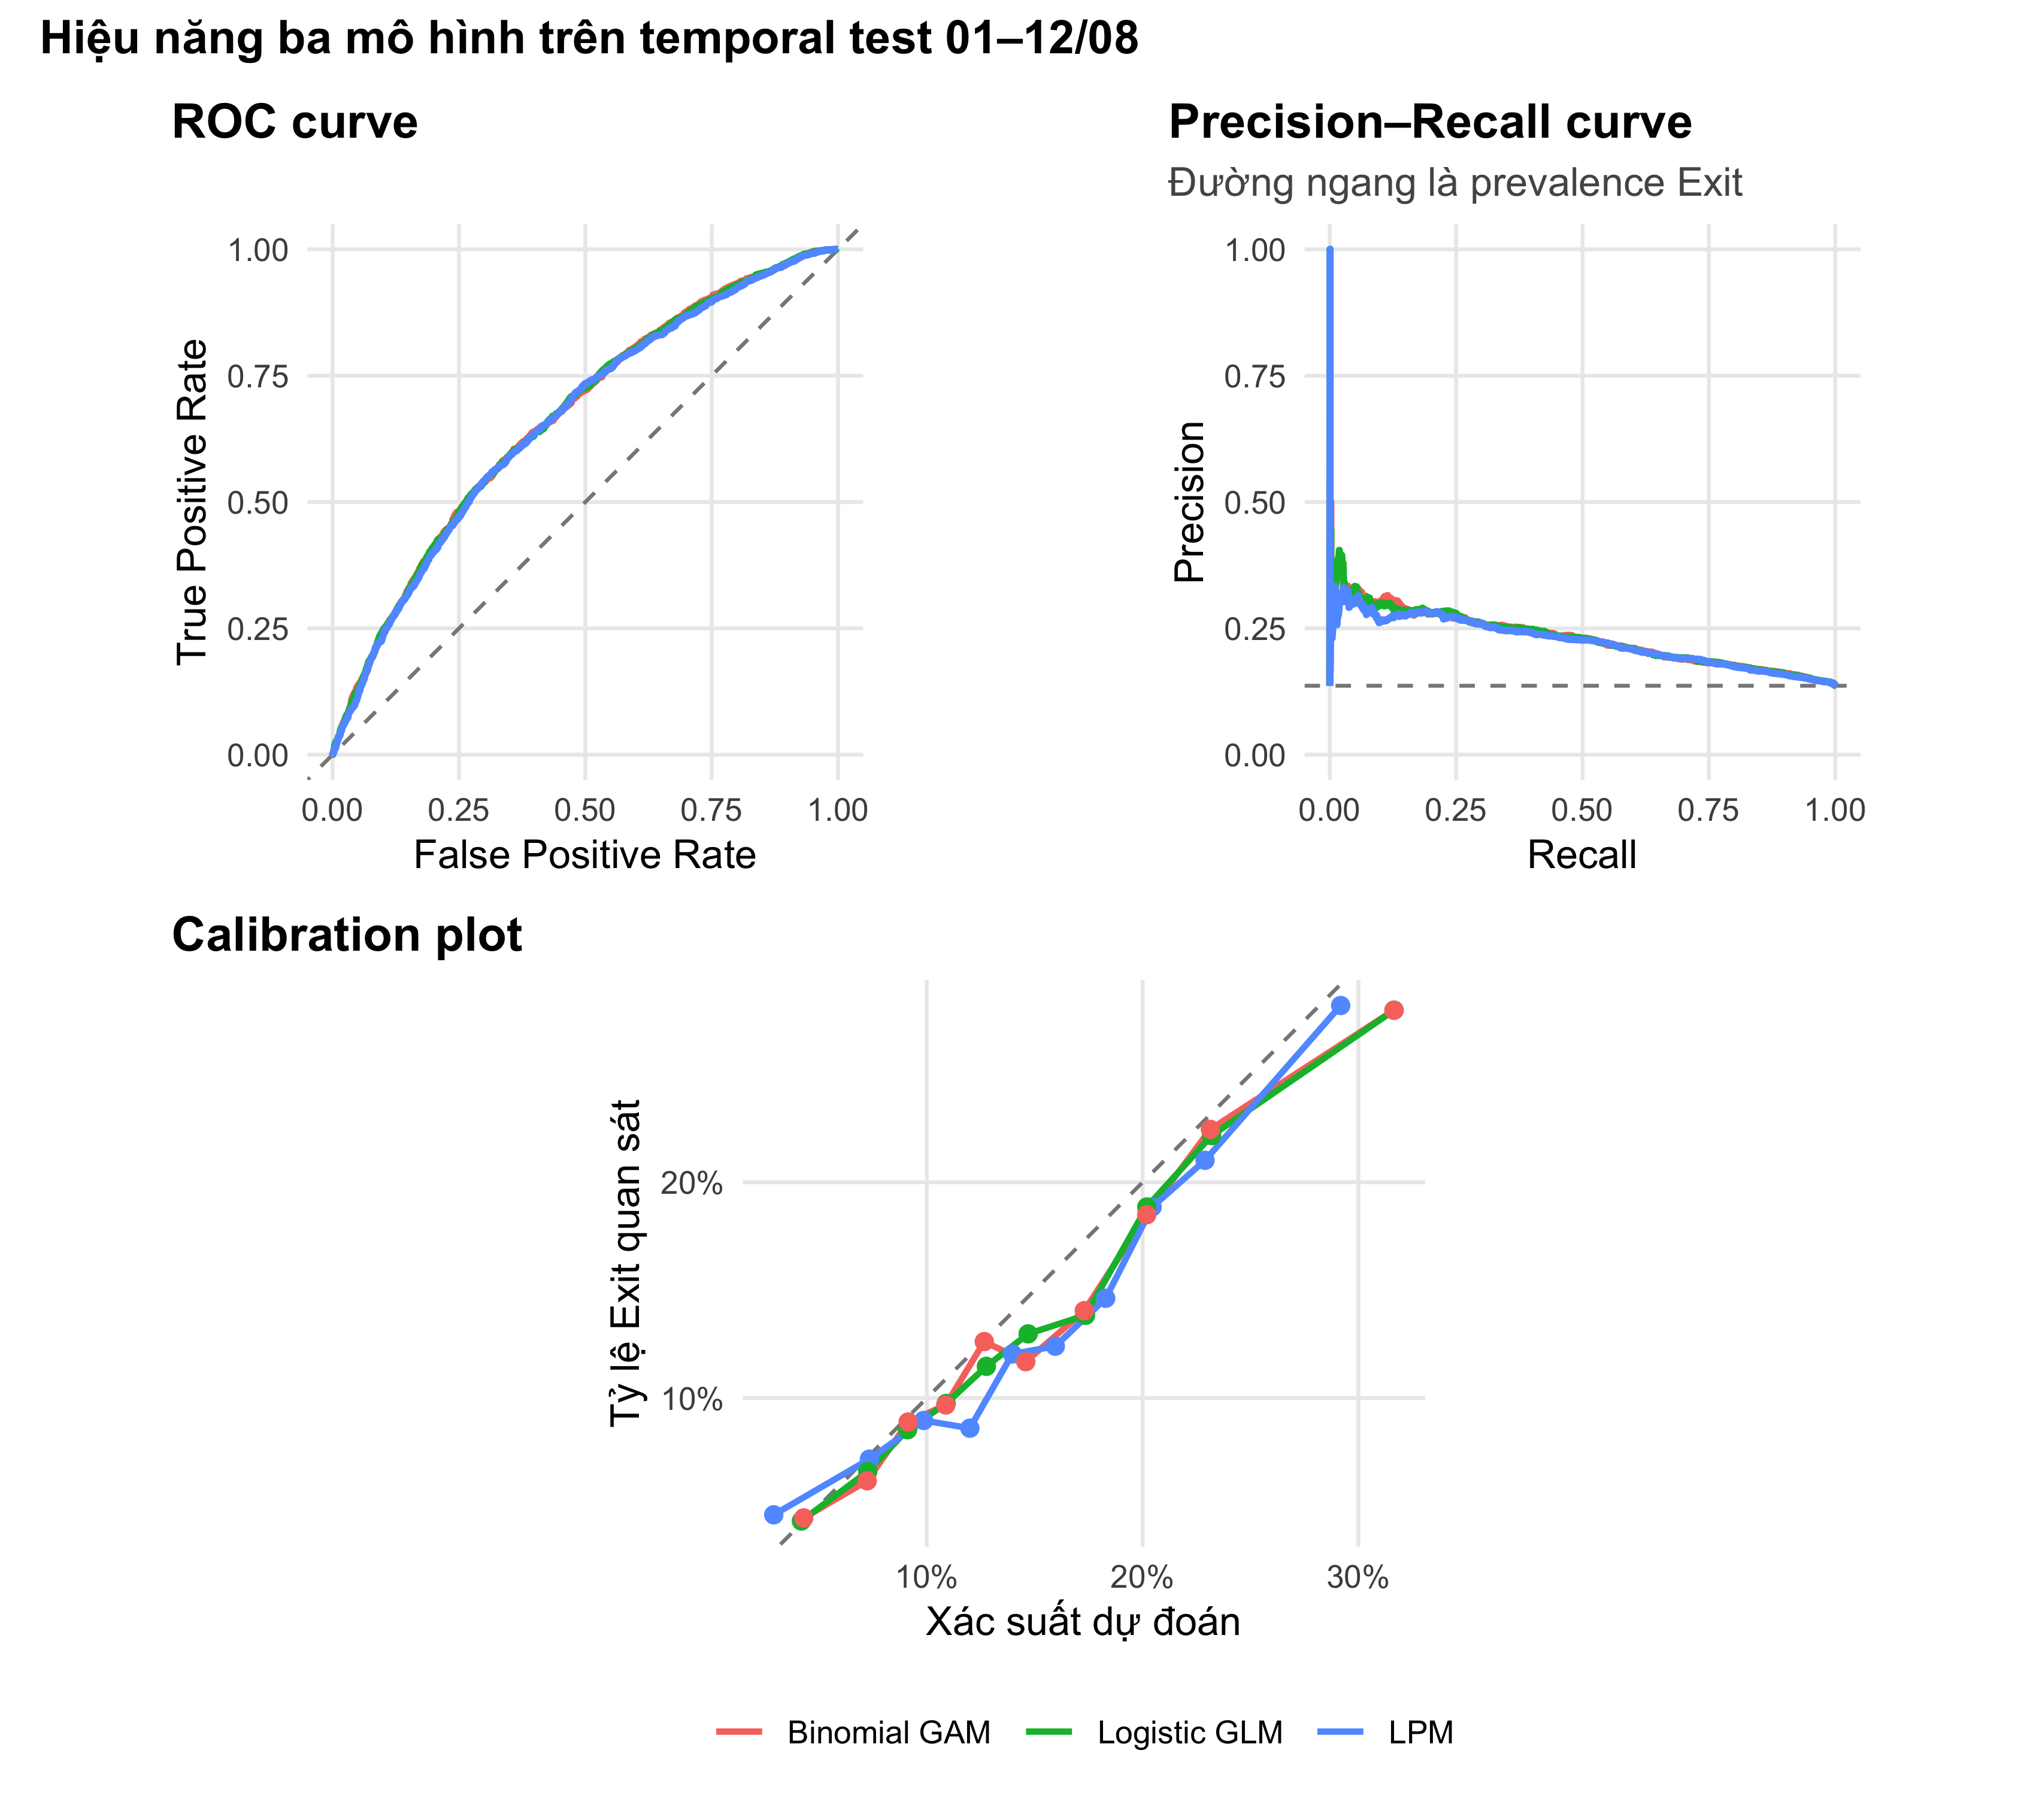
\includegraphics[width=0.95\textwidth]{img/fig-roc-pr-calibration.png}
\caption{Đường ROC, đường Precision--Recall và calibration plot của ba mô hình
trên temporal test 01--12/08. Đường đứt nét là mốc tham chiếu: xếp hạng ngẫu
nhiên (ROC), prevalence Exit (PR) và hiệu chỉnh hoàn hảo (calibration)}
\label{fig:roc-pr-calibration}
\end{figure}

\begin{table}[H]
\centering
\caption{Ma trận nhầm lẫn và các metric phân loại trên temporal test, tại
threshold đã khóa từ prediction out-of-fold của train}
\label{tab:classification}
\small
\setlength{\tabcolsep}{5pt}
\begin{tabular}{lrrrrrrrrrr}
\toprule
\textbf{Model} & \textbf{Threshold} & \textbf{TP} & \textbf{TN} & \textbf{FP}
& \textbf{FN} & \textbf{Accuracy} & \textbf{Precision} & \textbf{Recall}
& \textbf{Specificity} & \textbf{F1} \\
\midrule
LPM          & 0,168 & 1.176 & 7.428 & 4.617 & 727 & 61,69\% & 20,30\% & 61,80\% & 61,67\% & 30,56\% \\
Logistic GLM & 0,162 & 1.145 & 7.722 & 4.323 & 758 & 63,57\% & 20,94\% & 60,17\% & 64,11\% & 31,07\% \\
Binomial GAM & 0,163 & 1.123 & 7.843 & 4.202 & 780 & 64,28\% & 21,09\% & 59,01\% & 65,11\% & 31,07\% \\
\bottomrule
\end{tabular}
\end{table}

Các threshold được chọn (0,162--0,168) đều thấp hơn 0,5 rất nhiều, đúng như kỳ
vọng với dữ liệu mất cân bằng. Tại các ngưỡng này, cả ba mô hình đều có
Recall khoảng 59--62\% nhưng Precision chỉ khoảng 21\%: cứ 5 click bị dự báo là
kết thúc thì chỉ khoảng 1 click thực sự kết thúc. $F_1$ tối đa chỉ đạt 31,07\%.
Accuracy từ 61,69\% đến 64,28\% \emph{thấp hơn} mức 85,48\% mà một mô hình luôn dự đoán
``Continue'' đạt được -- minh chứng cụ thể cho lý do Accuracy không được dùng làm
tiêu chí chọn mô hình ở đây.

%\newpage
% Nội dung phần 4: Nhận xét và kết luận.

\section{Nhận xét và kết luận}

\subsection{Nhận xét về kết quả phân tích}

\subsubsection{Mô hình nào hoạt động tốt nhất và tại sao}

Theo quy tắc lựa chọn được chốt trước khi mở dữ liệu đánh giá,
\textbf{Logistic GLM với tầng predictor history-enhanced} là mô hình được chọn.
Lý do không nằm ở khả năng phân biệt -- về mặt này ba mô hình gần như không phân
biệt được, với ROC--AUC trên temporal test lần lượt là 0,662 (LPM), 0,666
(Logistic GLM) và 0,666 (Binomial GAM), các khoảng tin cậy bootstrap chồng lấn
gần hoàn toàn (Bảng~\ref{tab:final-metrics}).

Sự khác biệt thực chất nằm ở ba tiêu chí còn lại:

\begin{itemize}
  \item \textbf{Tính hợp lệ của xác suất.} LPM tạo ra 1,706\% dự đoán nằm ngoài
  khoảng $[0,1]$ trên temporal test -- những giá trị không thể diễn giải như xác
  suất. Logistic GLM và Binomial GAM theo cấu trúc không bao giờ mắc lỗi này.

  \item \textbf{Calibration.} Calibration slope của LPM chỉ đạt 0,868, trong khi
  Logistic GLM đạt 0,934 và GAM đạt 0,942 (lý tưởng là 1). Xác suất do LPM sinh
  ra cực đoan hơn mức dữ liệu thực sự cho phép.

  \item \textbf{Khả năng diễn giải và độ phức tạp.} Logistic GLM và Binomial GAM
  cho log loss (0,379) và Brier (0,113) giống nhau đến ba chữ số thập phân, tức
  GAM \emph{không} mua thêm được gì bằng độ phức tạp của nó. Thêm vào đó,
  concurvity giữa các term của GAM lên tới 0,994 (Bảng~\ref{tab:collinearity}),
  khiến các hàm trơn của nó không thể diễn giải riêng lẻ. Ngược lại, GVIF điều
  chỉnh lớn nhất của Logistic GLM chỉ 2,424, nên các hệ số của nó đọc được.
\end{itemize}

Sự tương đương giữa GAM và mô hình tuyến tính có một lý giải rõ ràng từ dữ liệu:
sau phép biến đổi $\log_2(\texttt{order})$, quan hệ giữa tiến trình session và
xác suất kết thúc đã gần như tuyến tính. Hình~\ref{fig:order-probability} cho
thấy ba đường dự đoán trùng nhau trong khoảng \texttt{order} từ 1 đến 20, và
Bảng~\ref{tab:kcheck} cho thấy các hàm trơn của biến giá chỉ có
$\text{edf} \approx 1$--$2$, tức gần như là đường thẳng. Nói cách khác, phần phi
tuyến mà GAM có thể khai thác trong bộ dữ liệu này là rất nhỏ.

\subsubsection{Các biến có ảnh hưởng lớn nhất}

Dựa trên kiểm định Wald robust theo cụm session (Bảng~\ref{tab:terms}), năm nhóm
biến có bằng chứng liên hệ mạnh nhất với \texttt{Exit} là
$\log_2(\text{Order})$, số danh mục duy nhất đã xem, hành vi quay lại sản phẩm
cũ, \texttt{Page} và \texttt{Country}. Ba hiệu ứng đáng chú ý nhất về độ lớn:

\begin{itemize}
  \item Click vào một sản phẩm \emph{đã xem trước đó} trong cùng session làm odds
  kết thúc tăng gấp 2,218 lần (CI 95\%: 2,064--2,384) -- hiệu ứng đơn biến mạnh
  nhất trong mô hình.
  \item Mỗi danh mục mới được xem thêm làm odds kết thúc nhân với 1,562
  (CI 95\%: 1,509--1,617).
  \item Ngược chiều, mỗi lần \texttt{order} tăng gấp đôi làm odds kết thúc nhân
  với 0,640 (CI 95\%: 0,623--0,657): session càng đi sâu thì càng ít khả năng
  dừng ở click kế tiếp.
\end{itemize}

Một phát hiện có giá trị phương pháp luận là \textbf{nhóm biến lịch sử duyệt quan
trọng hơn hẳn đặc điểm sản phẩm}. Thêm toàn bộ giá, danh mục, màu sắc, vị trí
ảnh, kiểu ảnh và trang hiển thị chỉ nâng ROC--AUC từ 0,589 lên 0,611; trong khi
nhóm biến lịch sử nâng tiếp lên 0,662 -- đóng góp hơn gấp đôi về ROC--AUC và gấp
ba lần về log loss. Cả hai bước
đều có robust joint $p < 0{,}001$, nhưng ý nghĩa thống kê và độ lớn thực tế là
hai chuyện khác nhau, và ở đây độ lớn nghiêng hẳn về nhóm biến hành vi.

Riêng \texttt{Price} tuy đạt ý nghĩa thống kê ($p = 0{,}008$) nhưng hiệu ứng rất
nhỏ (OR 1,032 cho mỗi 10 USD). Với cỡ mẫu 116.095 click của tập train, ngay cả
những liên hệ rất yếu cũng dễ đạt $p < 0{,}05$; vì vậy nhóm nhất quán đọc p-value
cùng với độ lớn hiệu ứng và khoảng tin cậy.

\subsubsection{Kết luận về kiểm định hai nhóm giá}

Ở mức ý nghĩa $\alpha = 0{,}05$, nhóm \textbf{bác bỏ giả thuyết $H_0$}: xác suất
\texttt{Exit} của hai nhóm giá không bằng nhau. Bằng chứng đến từ nhiều nguồn
nhất quán:

\begin{itemize}
  \item Kiểm định hai tỷ lệ thô: $\chi^2 = 10{,}08$, $p = 0{,}002$.
  \item Adjusted odds ratio với sai số chuẩn cluster-robust theo session:
  1,071 (CI 95\%: 1,002--1,144), $p = 0{,}043$.
  \item Chênh lệch thô 1,19 điểm phần trăm với cluster-bootstrap CI 95\% từ 0,46
  đến 1,93 điểm phần trăm -- không chứa 0.
  \item Cùng dấu và độ lớn tương đương trên cả ba giai đoạn thời gian
  (Bảng~\ref{tab:ab-temporal}).
\end{itemize}

Tuy nhiên, kết luận này cần ba dè dặt quan trọng. \emph{Thứ nhất}, độ lớn hiệu
ứng rất nhỏ: adjusted risk difference chỉ 0,82 điểm phần trăm với cận dưới khoảng
tin cậy là 0,03 -- gần như chạm 0. \emph{Thứ hai}, hiệu ứng không đồng đều giữa
các danh mục: sau hiệu chỉnh Holm chỉ riêng Trousers còn có ý nghĩa (2,32 điểm
phần trăm, $p = 0{,}008$), còn Skirts, Blouses và Sale đều có khoảng tin cậy chứa
0, với kiểm định tương tác nằm ngay ranh giới ($p = 0{,}051$). \emph{Thứ ba} và
quan trọng nhất, balance diagnostics (Hình~\ref{fig:ab-balance}) xác nhận hai
nhóm không tương đương như trong một thí nghiệm ngẫu nhiên. Đây là dữ liệu quan
sát, nên kết quả chỉ chứng minh một \textbf{mối liên hệ}, hoàn toàn không chứng
minh rằng việc tăng giá \emph{gây ra} việc kết thúc session.

\subsection{Kết luận tổng thể và khuyến nghị}

\subsubsection{Những hiểu biết rút ra}

\textbf{1. Rủi ro rời bỏ tập trung ở đầu session.} Xác suất kết thúc giảm từ
20,47\% tại click đầu tiên xuống 7,64\% sau click thứ 20 -- giảm hơn một nửa
(Bảng~\ref{tab:hazard}). Người dùng vượt qua được vài click đầu có xu hướng ở lại
lâu hơn nhiều.

\textbf{2. Hành vi trong phiên nói nhiều hơn thuộc tính sản phẩm.} Biết người
dùng \emph{đã làm gì} trong session (đã xem bao nhiêu danh mục, có quay lại sản
phẩm cũ không, có nhảy trang không) dự báo tốt hơn hẳn việc biết họ \emph{đang
xem sản phẩm nào}.

\textbf{3. Quay lại sản phẩm cũ là tín hiệu cảnh báo mạnh nhất.} Odds kết thúc
tăng gấp 2,218 lần. Cần lưu ý đây là quan hệ hai chiều về mặt diễn giải: hành vi
này vừa có thể là dấu hiệu người dùng đã tìm được thứ cần và sắp rời đi, vừa có
thể là dấu hiệu họ đang loanh quanh không tìm thấy gì mới. Dữ liệu hiện có không
phân biệt được hai kịch bản này vì thiếu thông tin giao dịch.

\textbf{4. Nhưng khả năng dự báo tổng thể còn hạn chế.} Đây là kết luận trung
thực cần nêu rõ: ROC--AUC 0,666 chỉ ở mức trung bình, Brier Skill Score 0,039
nghĩa là mô hình chỉ tốt hơn dự báo hằng khoảng 4\%, và tại threshold tối ưu
$F_1$ thì Precision chỉ 20,94\% -- cứ 5 cảnh báo thì khoảng 1 cảnh báo đúng.
Nguyên nhân chính là dữ liệu thiếu những tín hiệu quan trọng nhất: thời lượng
dừng lại trên mỗi trang, thao tác thêm vào giỏ hàng, và lịch sử người dùng qua
nhiều phiên.

\subsubsection{Khuyến nghị hành động}

\textbf{Về mặt vận hành:}

\begin{enumerate}
  \item \textbf{Ưu tiên can thiệp ở vài click đầu tiên.} Vì gần một phần năm
  session kết thúc ngay sau click đầu, các nỗ lực cải thiện trải nghiệm nên tập
  trung vào trang đầu tiên người dùng nhìn thấy. Lưu ý \texttt{Order} là một chỉ
  báo về giai đoạn session, không phải một biến có thể can thiệp trực tiếp.

  \item \textbf{Tính các đặc trưng hành vi theo thời gian thực.} Số sản phẩm và
  danh mục đã xem, cờ quay lại sản phẩm cũ, cờ chuyển danh mục -- toàn bộ đều
  tính được ngay tại click hiện tại mà không cần biết tương lai của session, nên
  triển khai được trong hệ thống trực tuyến.

  \item \textbf{Không tự động hóa quyết định dựa trên mô hình hiện tại.} Với
  Precision khoảng 21\%, việc tự động kích hoạt ưu đãi cho mọi phiên bị dự báo
  ``sắp rời'' sẽ lãng phí phần lớn ngân sách. Nếu dùng, chỉ nên dùng như một tín
  hiệu xếp hạng ưu tiên trong một hệ thống có chi phí can thiệp thấp.

  \item \textbf{Theo dõi calibration khi triển khai, không chỉ AUC.} Calibration
  intercept trên temporal test là $-0{,}127$, âm hơn so với mức $-0{,}059$ trên
  validation, cho thấy chất lượng xác suất suy giảm theo thời gian ngay cả khi
  AUC giữ nguyên. Mô hình cần được hiệu chỉnh lại định kỳ.
\end{enumerate}

\textbf{Về mặt thu thập dữ liệu:} giá trị gia tăng lớn nhất không đến từ mô hình
phức tạp hơn mà đến từ dữ liệu tốt hơn. Ba trường cần bổ sung, theo thứ tự ưu
tiên, là: dấu thời gian đầy đủ của từng click (để tính thời lượng dừng), sự kiện
thêm vào giỏ hàng và mua hàng (để chuyển từ dự báo ``rời phiên'' sang dự báo
``chuyển đổi''), và định danh người dùng xuyên phiên.

\textbf{Về nhóm giá:} không nên thay đổi chính sách giá dựa trên kết quả của báo
cáo này. Bằng chứng thu được là liên hệ trên dữ liệu quan sát, với độ lớn nhỏ và
không đồng đều giữa các danh mục. Bước đi đúng đắn là chạy một thí nghiệm ngẫu
nhiên thực sự theo thiết kế được trình bày ở Mục~\ref{subsec:future-ab}.

%\newpage
% Nội dung phần 5: Hạn chế và hướng phát triển.

\section{Hạn chế và hướng phát triển}

\subsection{Hạn chế của phân tích}

\subsubsection{Hạn chế về thiết kế nghiên cứu}

\begin{itemize}
  \item \textbf{Không có treatment/control ngẫu nhiên.} So sánh hai nhóm giá là
  phân tích quan sát. Balance diagnostics (Hình~\ref{fig:ab-balance}) cho thấy
  nhiều covariate có $|\text{SMD}| > 0{,}1$, tức hai nhóm khác nhau một cách hệ
  thống ngay từ đầu. Việc điều chỉnh bằng mô hình chỉ xử lý được các yếu tố đã
  quan sát; residual confounding bởi đặc điểm sản phẩm, danh mục và thói quen
  duyệt vẫn có thể tồn tại.

  \item \textbf{Giả thuyết được định hướng từ EDA.} Nhóm giá trở thành đối tượng
  kiểm định sau khi quan sát dữ liệu, không phải trước đó. Vì vậy p-value trong
  báo cáo cần được đọc cùng effect size, balance diagnostics, kiểm tra ổn định
  theo thời gian và hiệu chỉnh Holm, chứ không đứng một mình.

  \item \textbf{Quan hệ theo \texttt{Order} chịu cấu trúc chọn lọc.} Tại mỗi vị
  trí $t$, chỉ những session còn tồn tại đến $t$ được quan sát. Xu hướng giảm của
  xác suất kết thúc theo tiến trình vì vậy trộn lẫn hai cơ chế: thay đổi hành vi
  thực sự và việc các session có xu hướng dừng sớm đã bị loại khỏi mẫu.
\end{itemize}

\subsubsection{Hạn chế về dữ liệu}

\begin{itemize}
  \item \textbf{Không có thông tin chuyển đổi.} Dữ liệu không ghi giao dịch, giỏ
  hàng hay thanh toán. Vì vậy \texttt{Exit} chỉ có nghĩa ``click cuối của
  session'', hoàn toàn không phân biệt được một phiên kết thúc vì mua hàng thành
  công với một phiên kết thúc vì thất vọng bỏ đi. Đây là hạn chế nghiêm trọng
  nhất đối với giá trị kinh doanh của mô hình.

  \item \textbf{Không có chiều thời gian trong phiên.} Không có giờ click và
  không có thời lượng giữa hai click liên tiếp -- những tín hiệu thường mạnh nhất
  trong bài toán dự báo rời bỏ. Mô hình vì vậy buộc phải thay thế bằng các đại
  lượng đếm (số sản phẩm, số danh mục đã xem).

  \item \textbf{Không có định danh người dùng xuyên phiên.} Không thể phân biệt
  khách quay lại với khách mới, cũng không thể xây dựng đặc trưng lịch sử dài hạn.

  \item \textbf{Phụ thuộc trong cụm.} Các click trong cùng một session không độc
  lập. Nhóm đã dùng cluster-robust covariance và cluster bootstrap theo session,
  nhưng đây chỉ là hiệu chỉnh cho suy luận, không mô hình hóa tường minh cấu trúc
  phụ thuộc; một mô hình hiệu ứng hỗn hợp hoặc survival có thể phù hợp hơn.

  \item \textbf{Tháng 8 không đầy đủ.} Dữ liệu dừng ở ngày 13/08 và riêng ngày
  này chỉ có 200 click nên đã bị loại. Temporal test vì vậy chỉ gồm 12 ngày với
  13.948 click, khiến khoảng tin cậy bootstrap khá rộng
  (Bảng~\ref{tab:final-metrics}).

  \item \textbf{Tính đại diện.} Dữ liệu từ năm 2008 và của một cửa hàng cụ thể ở
  Ba Lan. Giao diện thương mại điện tử, thiết bị truy cập và hành vi người dùng
  đã thay đổi rất nhiều; cần đánh giá lại toàn bộ trước khi áp dụng cho môi
  trường hiện tại.
\end{itemize}

\subsubsection{Hạn chế về mô hình}

\begin{itemize}
  \item \textbf{Concurvity cao trong GAM.} Mức concurvity lớn nhất giữa các term
  đạt 0,994 (Bảng~\ref{tab:collinearity}). Đây là lý do các partial-effect plot ở
  Hình~\ref{fig:gam-smooths} chỉ được dùng để mô tả dạng hàm, không được diễn
  giải như hiệu ứng riêng của từng biến.

  \item \textbf{Biến \texttt{product\_model} bị bỏ qua.} Với 217 mức, biến này
  không được đưa vào mô hình chính vì chưa có quy tắc gộp mức hiếm được kiểm
  chứng. Có thể vì vậy mà một phần thông tin về sản phẩm bị bỏ sót.

  \item \textbf{Khả năng phân biệt còn khiêm tốn.} ROC--AUC 0,666 và Brier Skill
  Score 0,039 chưa đủ để coi mô hình là một hệ thống sẵn sàng triển khai.
\end{itemize}

\subsection{Đề xuất một thí nghiệm A/B ngẫu nhiên thực sự}
\label{subsec:future-ab}

Để chuyển từ kết luận liên hệ sang kết luận nhân quả, cần một thí nghiệm được
thiết kế đúng. Nhóm đề xuất thiết kế sau.

\textbf{Đơn vị ngẫu nhiên hóa.} Randomize ở \emph{cấp session}, lưu
\texttt{experiment\_id} cho từng phiên và đảm bảo mỗi session chỉ thuộc đúng một
nhánh trong suốt vòng đời của nó. Ngẫu nhiên hóa ở cấp click sẽ vi phạm giả định
độc lập vì các click trong cùng phiên phụ thuộc nhau.

\textbf{Treatment.} Thay vì tùy tiện thay đổi giá sản phẩm -- điều vừa rủi ro về
doanh thu vừa khó hoàn tác -- treatment khả thi hơn là cách \emph{trình bày}
thông tin giá:

\begin{itemize}
  \item \textbf{Control:} giao diện hiển thị giá hiện tại.
  \item \textbf{Treatment:} bổ sung thông điệp giá trị hoặc ưu đãi vận chuyển,
  giữ nguyên giá sản phẩm.
\end{itemize}

\textbf{Outcome.} Primary outcome là tỷ lệ session kết thúc trong một cửa sổ
click được xác định trước (ví dụ trong vòng 3 click kể từ khi nhìn thấy
treatment). Secondary outcomes gồm độ dài session và số sản phẩm duy nhất đã xem.
Cửa sổ outcome phải được khóa \emph{trước} khi thu thập dữ liệu.

\textbf{Phân tích.} Intention-to-treat, kiểm định hai phía tại
$\alpha = 0{,}05$, không dừng sớm dựa trên p-value chưa điều chỉnh. Nếu cần theo
dõi giữa chừng, phải dùng thiết kế sequential có kiểm soát sai lầm loại I.

\textbf{Về cỡ mẫu.} Nhóm cố ý \emph{không} báo cáo một con số cỡ mẫu tính từ hai
tỷ lệ click quan sát ở Bảng~\ref{tab:ab-rate}. Lý do là thí nghiệm tương lai
randomize theo session và có estimand hoàn toàn khác (tỷ lệ ở cấp session, không
phải cấp click), nên đưa ra con số như vậy sẽ gây hiểu nhầm. Trước khi tính
power cần khóa bốn tham số: cửa sổ outcome, tỷ lệ nền ở cấp session, minimum
detectable effect có ý nghĩa kinh doanh, và mức hao hụt dự kiến. Cỡ mẫu sau đó
được tính trực tiếp theo số session mỗi nhánh.

\subsection{Hướng phát triển khác}

\begin{itemize}
  \item \textbf{Mô hình sinh tồn thời gian rời rạc.} Bài toán hiện tại về bản
  chất là ước lượng hazard rời rạc. Một mô hình survival có thể xử lý tường minh
  cấu trúc chọn lọc theo \texttt{Order} thay vì chỉ điều chỉnh gián tiếp.

  \item \textbf{Mô hình hiệu ứng hỗn hợp.} Thêm random intercept theo session sẽ
  mô hình hóa trực tiếp phần phụ thuộc trong cụm thay vì chỉ hiệu chỉnh sai số
  chuẩn.

  \item \textbf{Đối chứng bằng mô hình phi tham số.} Gradient boosting hoặc
  random forest có thể cho biết trần hiệu năng thực sự của bộ đặc trưng hiện tại;
  nếu chúng cũng chỉ đạt ROC--AUC quanh 0,67 thì giới hạn nằm ở dữ liệu chứ không
  ở dạng mô hình.

  \item \textbf{Gộp mức của \texttt{product\_model}.} Xây dựng quy tắc gộp 217 mã
  sản phẩm dựa trên tần suất trong tập train, rồi đánh giá phần thông tin bổ sung
  bằng đúng pipeline hiện tại.
\end{itemize}

%\newpage
% Nội dung phần 6: Phụ lục.

\section{Phụ lục}

\subsection{Hiệu năng phân tầng của mô hình được chọn}

Bảng~\ref{tab:subgroup} kiểm tra xem Logistic GLM có hoạt động đồng đều trên các
phân nhóm hay không, tính trên temporal test 01--12/08.

\begin{table}[H]
\centering
\caption{Hiệu năng phân tầng của Logistic GLM trên temporal test 01--12/08}
\label{tab:subgroup}
\small
\begin{tabular}{llrrrrrr}
\toprule
\textbf{Phân tầng} & \textbf{Nhóm} & \textbf{N} & \textbf{Prevalence}
& \textbf{ROC--AUC} & \textbf{AP} & \textbf{Log loss} & \textbf{Brier} \\
\midrule
\multirow{4}{*}{Category}
 & Trousers & 4.067 & 12,59\% & 0,638 & 0,200 & 0,365 & 0,107 \\
 & Skirts   & 2.769 & 15,57\% & 0,632 & 0,216 & 0,420 & 0,129 \\
 & Blouses  & 3.205 & 13,92\% & 0,688 & 0,252 & 0,380 & 0,114 \\
 & Sale     & 3.907 & 13,16\% & 0,693 & 0,252 & 0,364 & 0,108 \\
\midrule
\multirow{6}{*}{Order}
 & 1--2   & 3.437 & 18,10\% & 0,612 & 0,241 & 0,465 & 0,146 \\
 & 3--4   & 2.357 & 15,27\% & 0,616 & 0,233 & 0,418 & 0,127 \\
 & 5--7   & 2.395 & 13,70\% & 0,631 & 0,213 & 0,388 & 0,116 \\
 & 8--12  & 2.273 & 13,33\% & 0,664 & 0,261 & 0,370 & 0,110 \\
 & 13--20 & 1.653 & 9,13\%  & 0,670 & 0,198 & 0,292 & 0,080 \\
 & $>$20  & 1.833 & 7,58\%  & 0,723 & 0,187 & 0,245 & 0,066 \\
\bottomrule
\end{tabular}
\end{table}

Hiệu năng \emph{không} đồng đều giữa các phân nhóm. Theo danh mục, ROC--AUC dao
động từ 0,632 (Skirts) đến 0,693 (Sale). Theo tiến trình session, xu hướng rõ
ràng hơn: AUC tăng đều từ 0,612 ở khoảng \texttt{Order} 1--2 lên 0,723 với các
click sau vị trí 20. Nói cách khác, mô hình dự báo tốt hơn ở giai đoạn muộn của
phiên -- đúng lúc thông tin lịch sử duyệt đã tích lũy đủ. Đây cũng là hạn chế
thực tiễn: mô hình yếu nhất chính ở giai đoạn đầu, nơi rủi ro rời bỏ cao nhất.

Lưu ý rằng Brier score giảm dần theo \texttt{Order} chủ yếu vì prevalence giảm
(từ 18,10\% xuống 7,58\%), không phải vì mô hình tốt lên; hai chỉ số này phải đọc
cùng nhau.

\subsection{Phân công công việc}

\begin{table}[H]
\centering
\caption{Phân công công việc trong nhóm}
\label{tab:assignment}
\small
\begin{tabular}{>{\raggedright\arraybackslash}p{0.22\textwidth}
                >{\raggedright\arraybackslash}p{0.14\textwidth}
                >{\raggedright\arraybackslash}p{0.52\textwidth}}
\toprule
\textbf{Họ và tên} & \textbf{MSSV} & \textbf{Nội dung phụ trách} \\
\midrule
Nghi & 25C230XX &
Phần 1: giới thiệu bộ dữ liệu, xác định mục tiêu phân tích và xây dựng bản đề
xuất phương pháp; phối hợp viết Phần 4. \\[2pt]
Lê Hoàng Như & 25C23014 &
Phần 2: làm sạch dữ liệu, thống kê mô tả và trực quan hóa; phối hợp viết Phần 4;
soạn slide thuyết trình. \\[2pt]
Nguyễn Nhật Quang & 25C23002 &
Phần 3: xây dựng và đánh giá mô hình, toàn bộ bảng kết quả và biểu đồ; tổng hợp
nội dung hai file Rmd thành báo cáo nộp; phối hợp viết Phần 4. \\
\bottomrule
\end{tabular}
\end{table}

% TODO: cập nhật MSSV và họ tên đầy đủ của thành viên Nghi ở bảng trên
% và trong \studentname của file main.tex.

\subsection{Ghi chú về tính tái lập}

Toàn bộ kết quả trong báo cáo được sinh từ một lần render duy nhất của file
\texttt{de\_xuat\_phan\_tich\_clickstream.Rmd} bằng R~\cite{rcore2026} trong một
session sạch, không phụ thuộc vào object còn sót lại trong môi trường làm việc.

\begin{table}[H]
\centering
\caption{Môi trường thực thi}
\label{tab:environment}
\small
\begin{tabular}{ll}
\toprule
\textbf{Thành phần} & \textbf{Phiên bản} \\
\midrule
R           & 4.6.0 (2026-04-24) \\
rmarkdown   & 2.31 \\
knitr       & 1.51 \\
mgcv        & 1.9.4 \\
sandwich    & 3.1.1 \\
lmtest      & 0.9.40 \\
car         & 3.1.5 \\
dplyr       & 1.2.1 \\
tidyr       & 1.3.2 \\
ggplot2     & 4.0.3 \\
patchwork   & 1.3.2 \\
scales      & 1.4.0 \\
emmeans     & 2.0.4 \\
\bottomrule
\end{tabular}
\end{table}

\textbf{Nguồn dữ liệu.} File \texttt{e-shop clothing 2008.csv} (phân tách bằng
dấu chấm phẩy, 14 cột, 165.474 dòng), không chỉnh sửa thủ công.

\textbf{Seed ngẫu nhiên.} Mọi thủ tục có yếu tố ngẫu nhiên đều dùng
\texttt{set.seed(20260726)}: chia five-fold cross-validation theo session, 1.000
lần cluster bootstrap cho risk difference thô, và 500 lần cluster bootstrap cho
khoảng tin cậy của các metric trên temporal test. Nhờ vậy toàn bộ con số trong
báo cáo tái lập được chính xác.

\textbf{Kiểm tra tự động trong pipeline.} File Rmd chứa các khẳng định
\texttt{stopifnot()} được kiểm tra ở mỗi lần chạy: đúng 165.474 dòng và 24.026
session; không có giá trị khuyết thiếu hay dòng trùng lặp; \texttt{order} liên
tục trong mọi session; mỗi session có đúng một click \texttt{Exit = 1}; và không
có session nào xuất hiện đồng thời ở hai tập dữ liệu. Nếu bất kỳ điều kiện nào
sai, quá trình render sẽ dừng với lỗi thay vì tạo ra báo cáo không hợp lệ.

\textbf{Lệnh render.} Chạy từ thư mục chứa file Rmd và file CSV:

\begin{lstlisting}[language=R]
rmarkdown::render(
  "de_xuat_phan_tich_clickstream.Rmd",
  params = list(show_code = FALSE),
  envir  = new.env()
)
\end{lstlisting}

Tham số \texttt{show\_code = FALSE} tạo bản nộp không hiển thị mã nguồn; đặt
\texttt{show\_code = TRUE} sẽ tạo bản kiểm tra có kèm mã R cho từng bảng và biểu
đồ. Các hình trong báo cáo LaTeX này được xuất ở độ phân giải 200 dpi từ đúng lần
chạy nói trên và lưu trong thư mục \texttt{img/} với tiền tố \texttt{fig-}.

% \input{content/hinhanh}
% \input{content/bangbieu}
% \input{content/congthuctoan}
% \input{content/thuattoan}
% \input{content/code}
% \input{content/ngonngu}
% \input{content/cite}

% Appendix
% \appendix
% Add \cleardoublepage to move appendices to next page.
% \input{appendix/appendix.tex}

\bibliographystyle{plain}
\bibliography{reference}

\end{document}
